\chapter{Solution Methodology}

\section{Introduction}
 The methodology for online stability prediction is is generalized using a flowchart shown in fig. \ref{Flowchart}. It is a long process but in my paper discussed portion is of only computation of indicators. So left out processes like fault detection, post fault data collection, stability analysis are carried out using MAT-POWER and MAT-TRANS Software. These softwares are discussed in following sections.\par
 After fault occurs the data are collected from PMU and Time-stamped measurements data generated from simulation. Then the data are sent for performing Stability Analysis. The Results are taken out for obtaining different required parameters, one of them is Coherency Referred measures
Computation, that includes Computation of Area Based COI,
System Based COI, then COI. After getting the parameters different Catastrophic Indicators are Computed one by
one to analyze them.
 
 \begin{figure}
	 \centering
	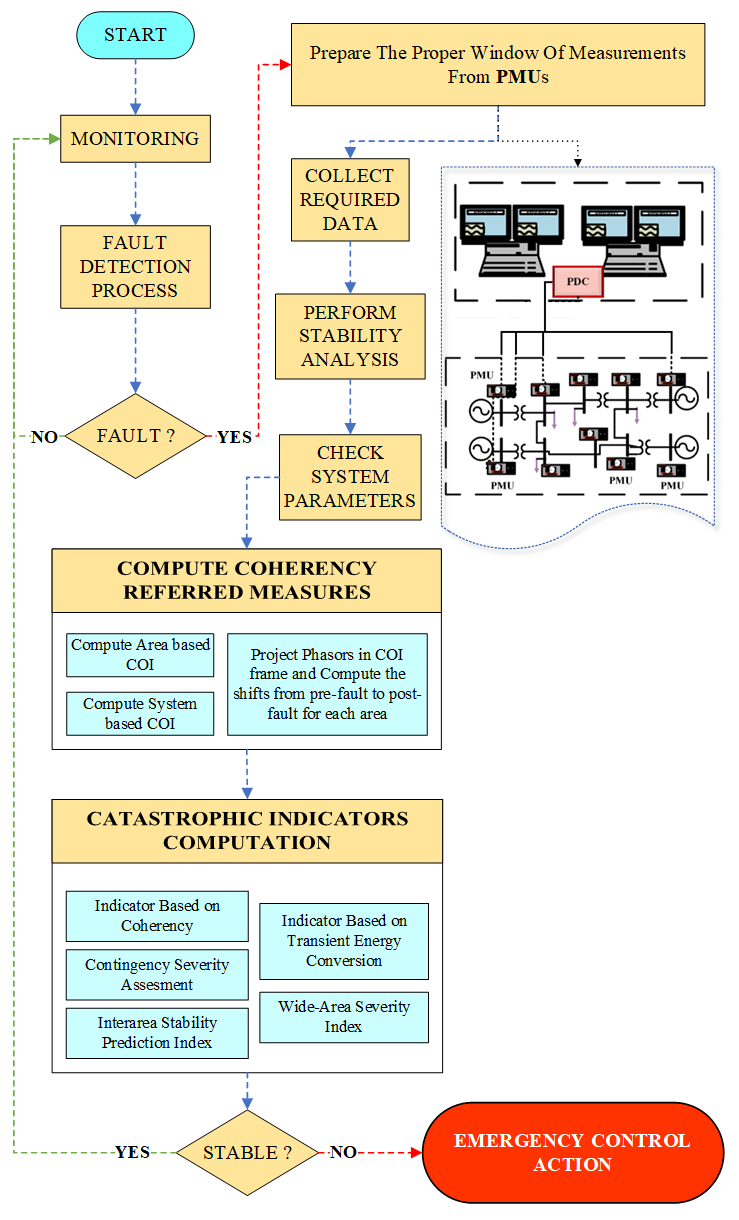
\includegraphics[width=12 cm]{Flowchart2.png}
	\caption{Flowchart of Stability Prediction Procedure}
	\label{Flowchart}
\end{figure} 

\section{MAT-POWER Tool Box}
 This Toolbox provides 59 built-in MATLAB programs for various famous test Systems. All these MATLAB programs of various test systems are shown in the DATA folder of the MAT-POWER toolbox, which can be directly used. It is expected as a simulation device for scientists and teachers that is not difficult to utilize and adjust. MAT-POWER is intended to give the most ideal exhibition while keeping the code easy to comprehend and adjust. Syntax for running the Optimal power Flow of a Case:- \textbf{runopf(‘casefilename’);} A simple example of MAT-POWER use can be described in following sub-section along with its result comparison with theoretical values.

\subsection{Economic Load Dispatch Example on IEEE-9 Bus System}
\begin{itemize} 
\item[\tiny{$\blacksquare$}]The M-file for IEEE-9 Bus test name is case9. So, the syntax for running optimal Power flow or Economic load Dispatch in IEEE-9 Bus system is \textbf{runopf('case9')}. By default it will perform the optimal power flow using MATPOWER Interior Point Solver(MIPS). 
\item[\tiny{$\blacksquare$}]It has taken the computational time of 3.06 seconds. Furthermore, the total minimum cost to supply the load of IEEE-9 Bus system is 5296.69 \$/hr. It further shows the important results of IEEE-9 bus system such as minimum and maximum voltage magnitudes, Voltage angle, active and reactive power loss and incremental fuel cost. Along with Total Power Supplied, Total Power Demand and Total Loss is also generated as 318.31 MW, 315.0 MW and 3.31 MW respectively.
\item[\tiny{$\blacksquare$}]The Mat-Power software testing is completed with Results and are compared and verified to be same as the Theoretical data.
\end{itemize}
\textbf{*Although there is no direct use of MAT-POWER Software, but the later proceedings need the presence of it along with MATLAB.}

\section{MAT-TRANS Software}
MATTRANS is a MATLAB(R)/Simulink (M-files and.mdl files) programme for transient stability analysis. It's a free and open-source programme. It's designed to be a simple to use and modify simulation tool for researchers and instructors. MATTRANS was created with the goal of providing the highest feasible performance while making the code simple to understand and modify. It was first created in 2008, and the files are available at\cite{MattransSoft}. In MATTRANS, the runts(case\#, case\#dd) function requires two.m input files. There are two types of network data: 1) steady-state data and 2) dynamic data. The network steady-state data format is identical to that of MATPOWER \cite{L1}, but the network dynamic data format contains variables for generator machines, exciters, turbines, and power system stability.

\subsection{Pseudo-Code of the MATTRANS Software}
This software Runs a Transient Stability. Where, mpc = 
runts(casedata, mpopt, fname, solvedcase). It runs a 
Transient Stability (First executes power flow then simulate transtability.mdl), returning results. Its software coading includes following steps-
\begin{enumerate}
\item Imports code files such as “import +data.*; import +exciter.*; import +generator.*; import +load.*; import +pss.*; import +turbine.*; import +utils.*; import +Yform.*; “ to include exciter data, generator data, load data and other important data’s with functions to carryout important logics for transient stability analysis.
\item Initializes named Indices for bus, generator and branch matrices.
\item	Executes steady-state power flow. moption used to set and retrieve a MATPOWER option structure runpf runs a power flow.
\item	Adding dynamic data to the mpc structure and adding extra variables but gen, order variables are removed from mpc as they are already included in the Simulink file.
\item	Generator variables for a particular case data is included.
\item	Exciter variables are initialized and they are enabled or disabled according to corresponding generator.
\item	Turbine and speed governors values are initialized and they are enabled or disabled according to corresponding generator.
\item	Initialization of PSS Models and they are enabled or disabled according to the corresponding generators. This process includes initialization of PSS Models, selectors for individual type of PSS, Indication of the generator number of which specific type of PSS is to be enabled otherwise it is marked as zero and then wrapping up it into a single structure.
\item	Modelling Load variables include finding load variables and wrapping up it into a single structure to reduce complexity.
\item	Modelling Y-Bus w.r.t line trips includes necessary variable declaration, Y-bus formation, inclusion of dynamic data of both load and generator in Y-bus, input command line interface for users to enter fault data followed by condition for tripping of lines to clear fault and wrapping all data’s into a single structure.
\item	Execution of transientStability.mdl i.e. a Simulink file specially used for evaluation of above collected datas and shows parameter output for the indicators for assessment of stability.
\end{enumerate}

\subsection{Simulation Models}
Execution of transientStability.mdl includes the execution of the base model known as \textbf{Transient Stability model} shown in Fig. \ref{TSM} which also includes various sub models to check for Transient Stability of a system. Important sub models are \textbf{Generator, Turbine System, Excitation system, Power System Stability Model, Static Loads and its outputs}, which are discussed below. 
\begin{figure}[H]
	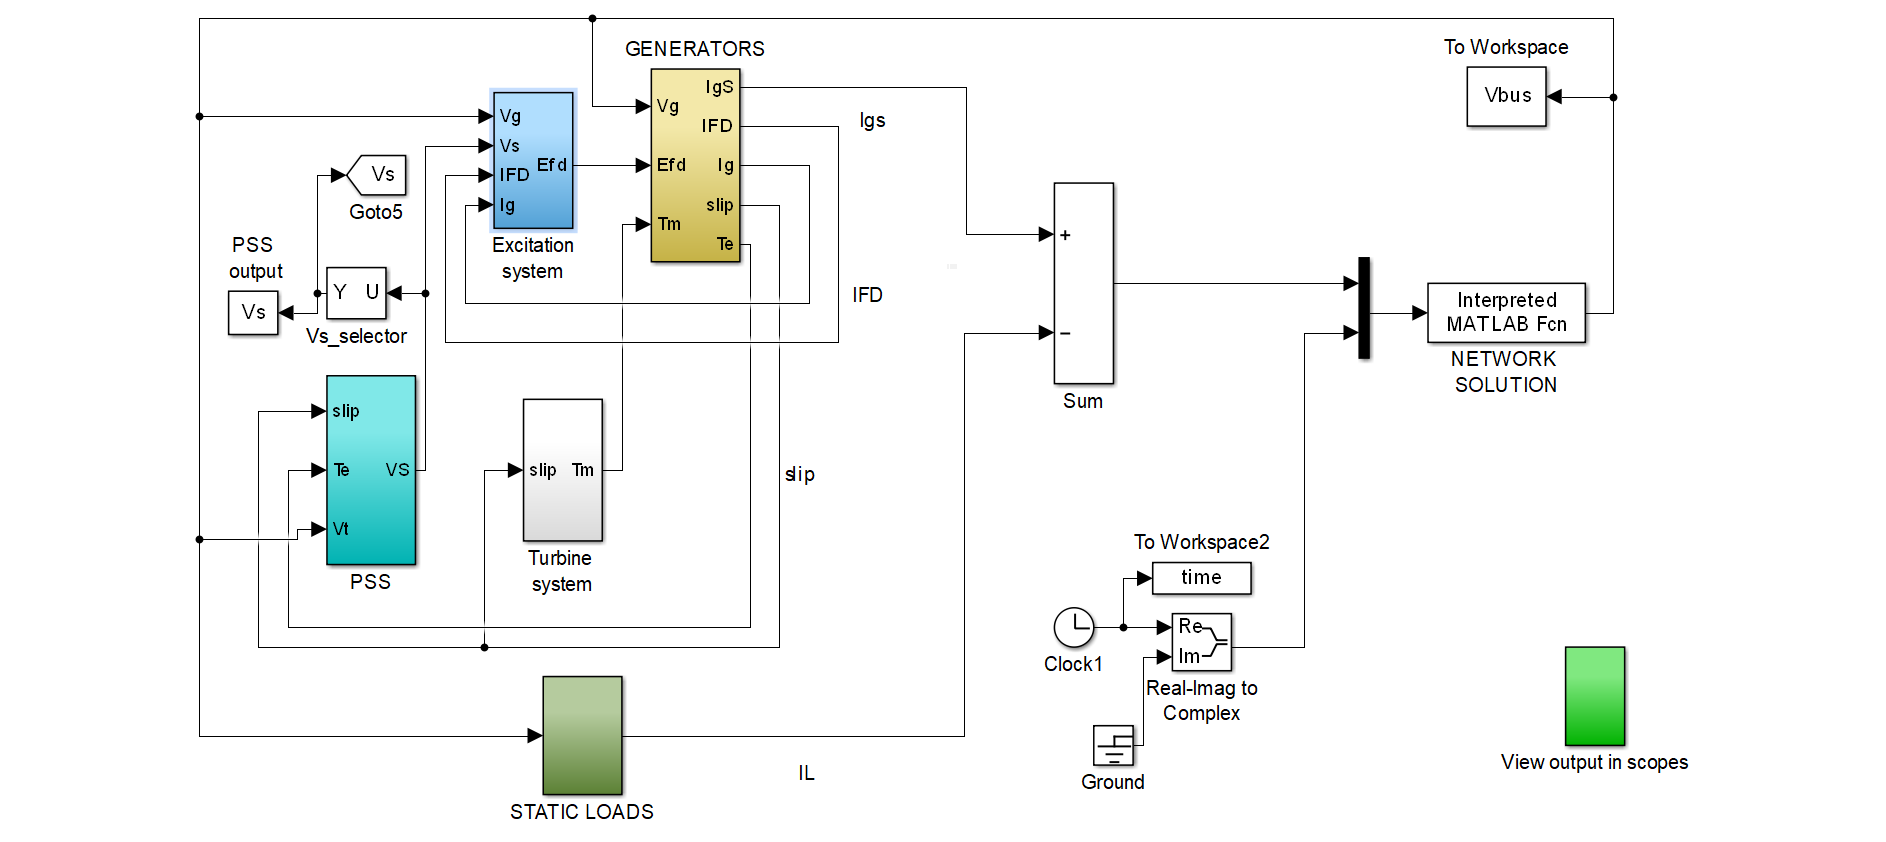
\includegraphics[scale=0.4]{Transient Stability}
	\caption{Transient Stability Model}
	\label{TSM}
	\end{figure}
	
\begin{enumerate}
%% 1. Generator Model==============================================================
\item \textbf{\large Generator Model}: It is created to do the work of a normal generator (Electric machine) shown in Fig. \ref{GM} and along with calculating its parameters like torque, angle deviation, field current, saliency etc..
	
	\begin{figure}[H]
	 \centering
	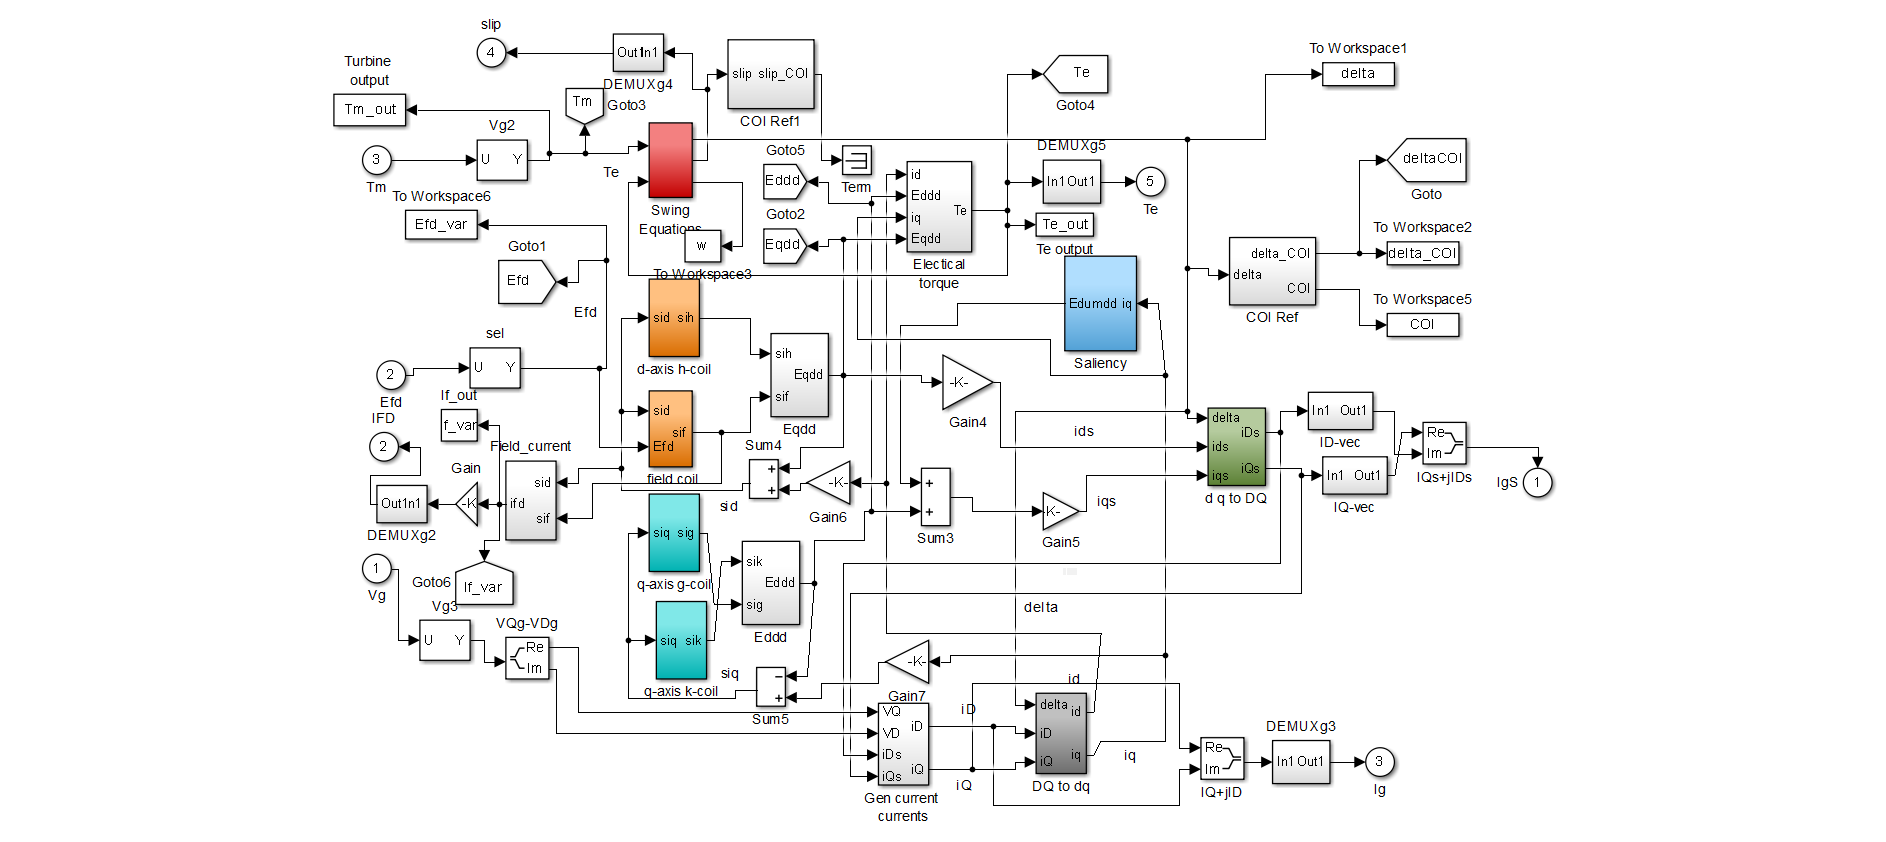
\includegraphics[scale=0.4]{Generators}
	\caption{Generator Model}
	\label{GM}
	\end{figure}
	% Generator Sub models-------------------------------------------------------
	\begin{itemize}
%		\item \textbf{\large Generator Sub Models}: Generator parts like Field Coil 			parameters, Direct axis parameters, Quadrature axis parameters, Saliency 				models are prepared for making a complete generator model and for 					calculating generator parameters and also COI Reference Model for obtaining 			generator speed Deviation.
%		\begin{figure}[H]
%		 \centering
%		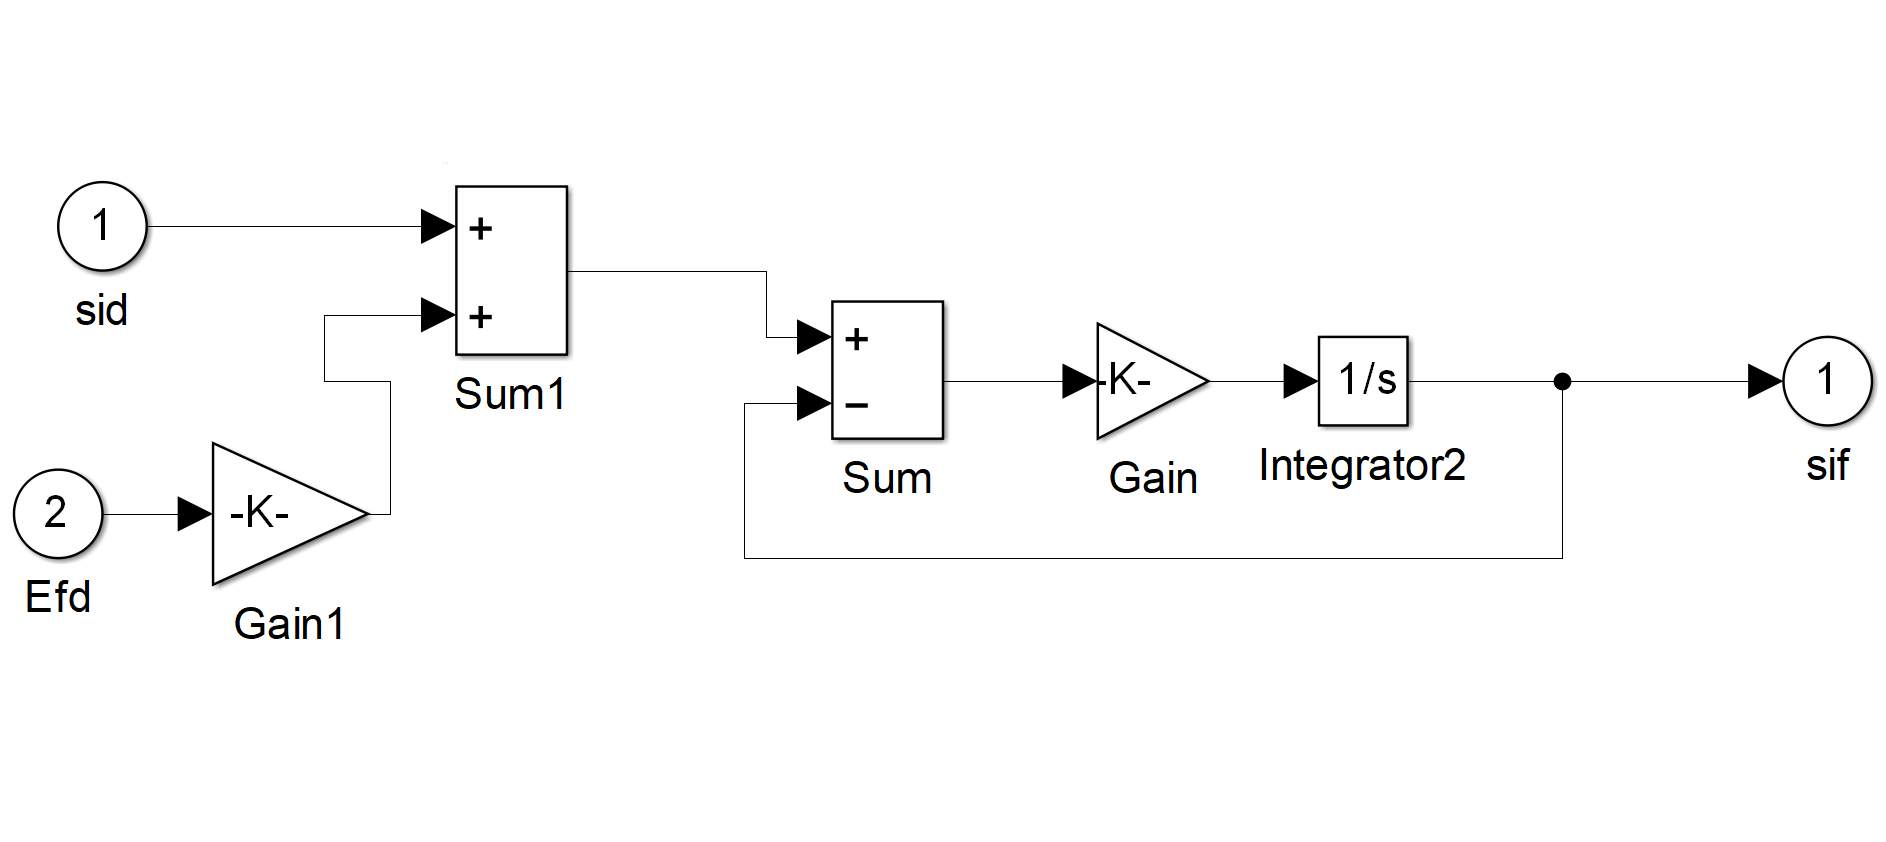
\includegraphics[scale=0.3]{Field Coil}
%		\caption{Field Coil Model}
%		\label{Field Coil}
%		\end{figure}
%		
%		\begin{figure}[H]
%		 \centering
%		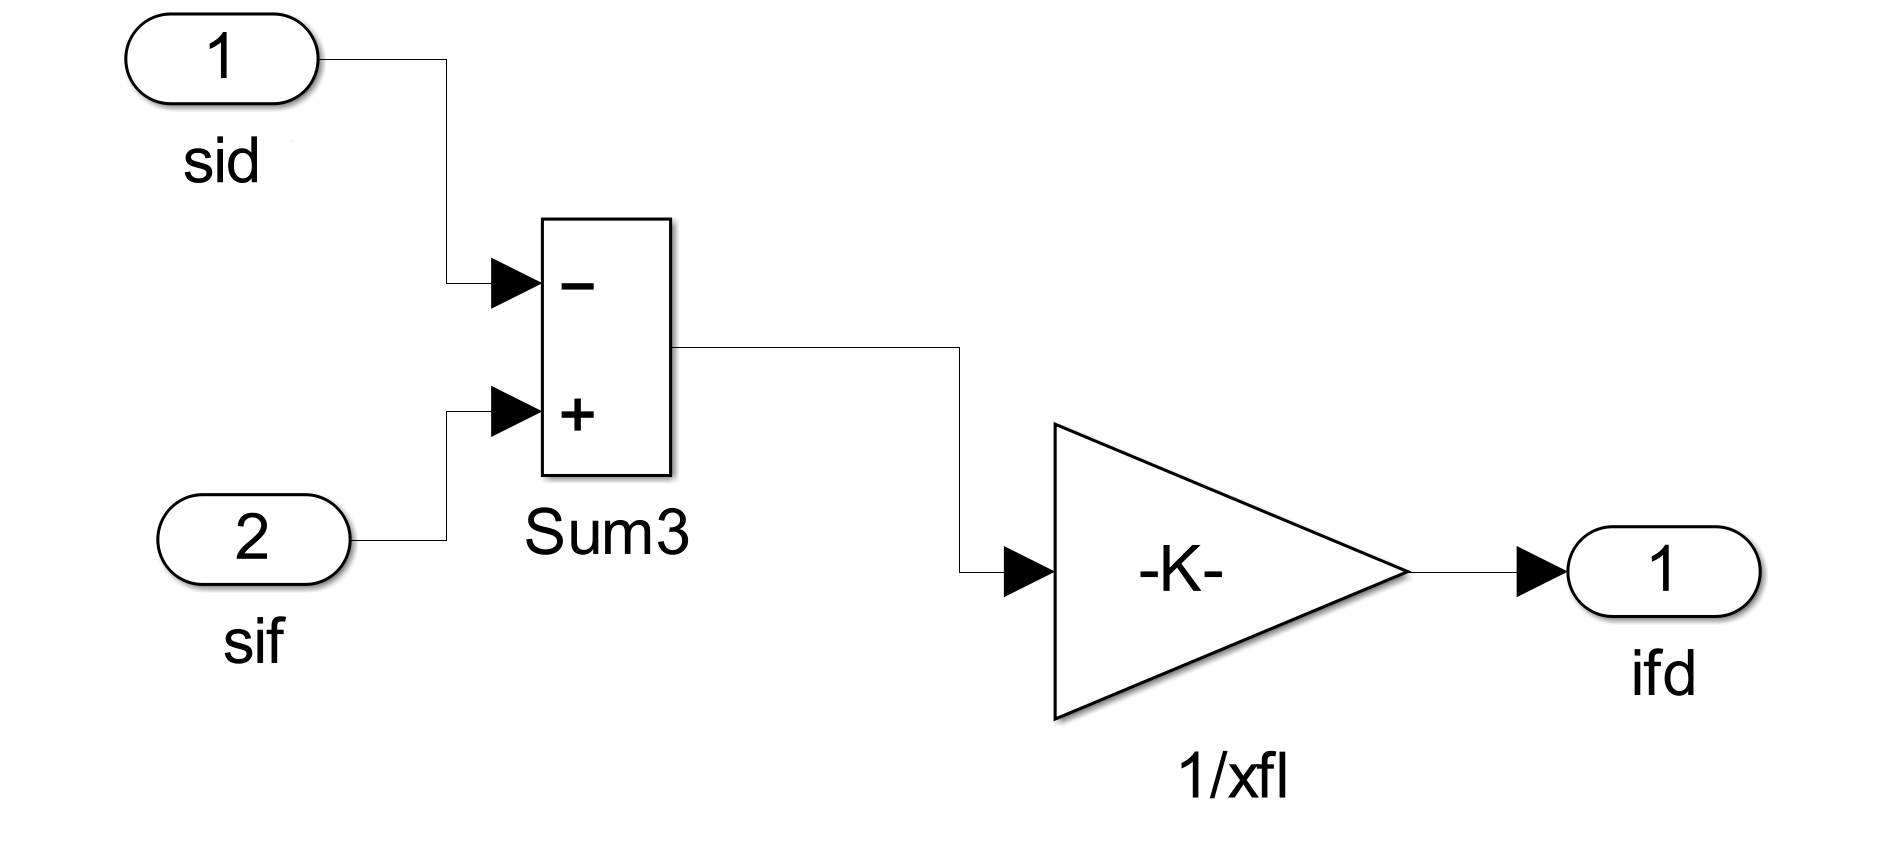
\includegraphics[scale=0.3]{Field Current}
%		\caption{Field Current Model}
%		\label{Field Current}
%		\end{figure}
%		
%		\begin{figure}[H]
%		 \centering
%		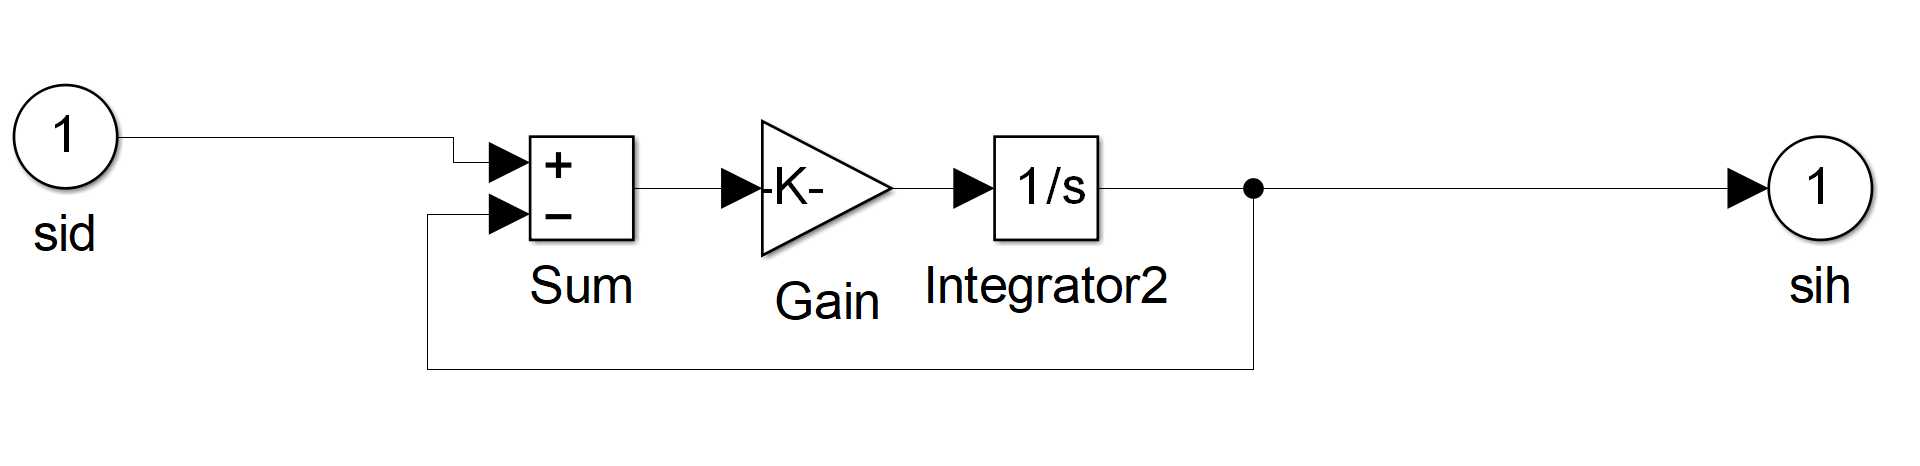
\includegraphics[scale=0.3]{d-axis h-coil}
%		\caption{d-axis h-coil Model}
%		\label{dh}
%		\end{figure}
%		
%		\begin{figure}[H]
%		 \centering
%		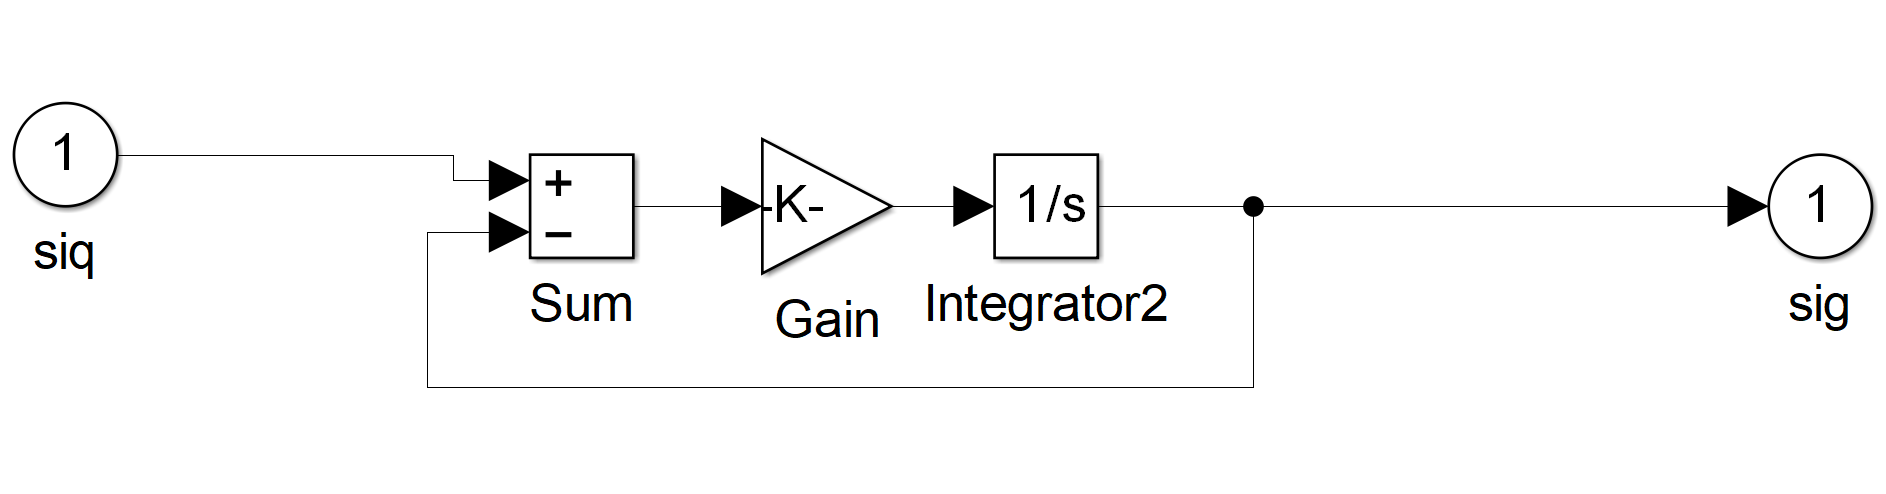
\includegraphics[scale=0.3]{q-axis g-coil}
%		\caption{q-axis g-coil Model}
%		\label{qh}
%		\end{figure}
%		
%		\begin{figure}[H]
%		 \centering
%		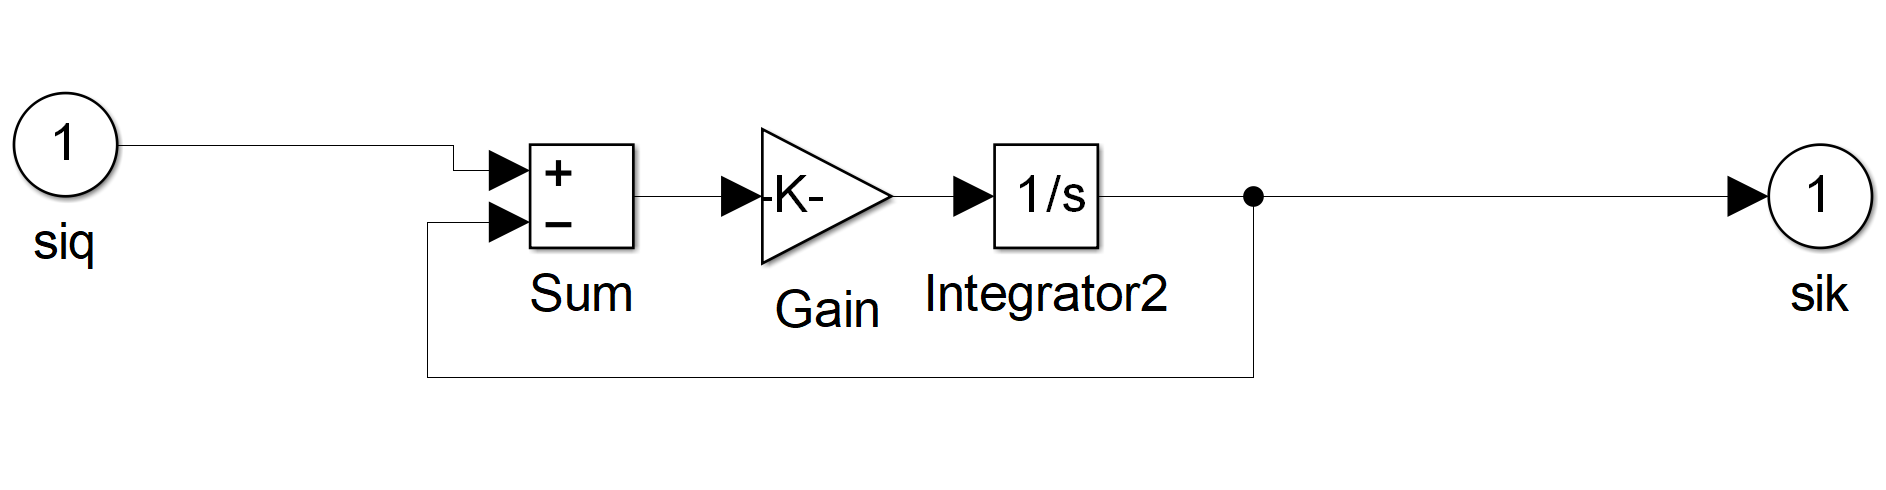
\includegraphics[scale=0.3]{q-axis k-coil}
%		\caption{q-axis k-coil Model}
%		\label{qk}
%		\end{figure}
%		
%		\begin{figure}[H]
%		 \centering
%		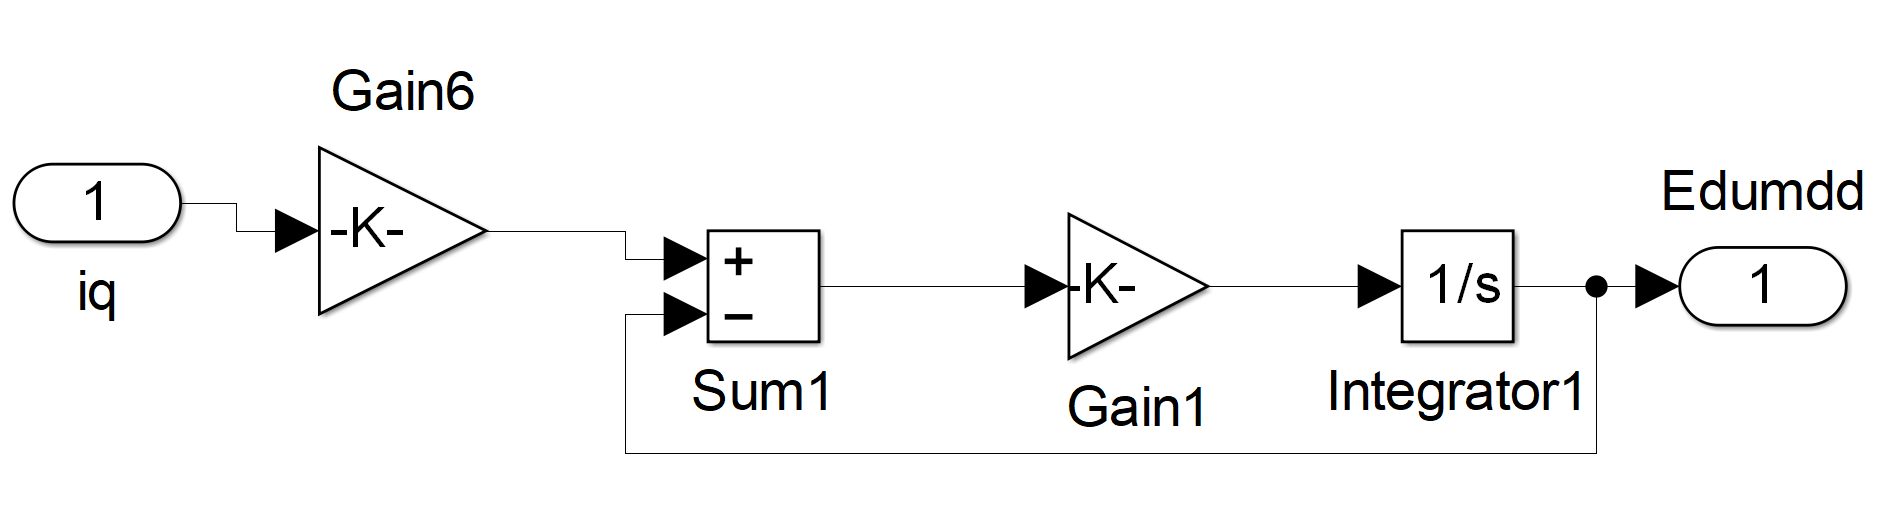
\includegraphics[scale=0.3]{Saliency}
%		\caption{Saliency Model}
%		\label{Saliency}
%		\end{figure}
%		
%		\begin{figure}[H]
%		 \centering
%		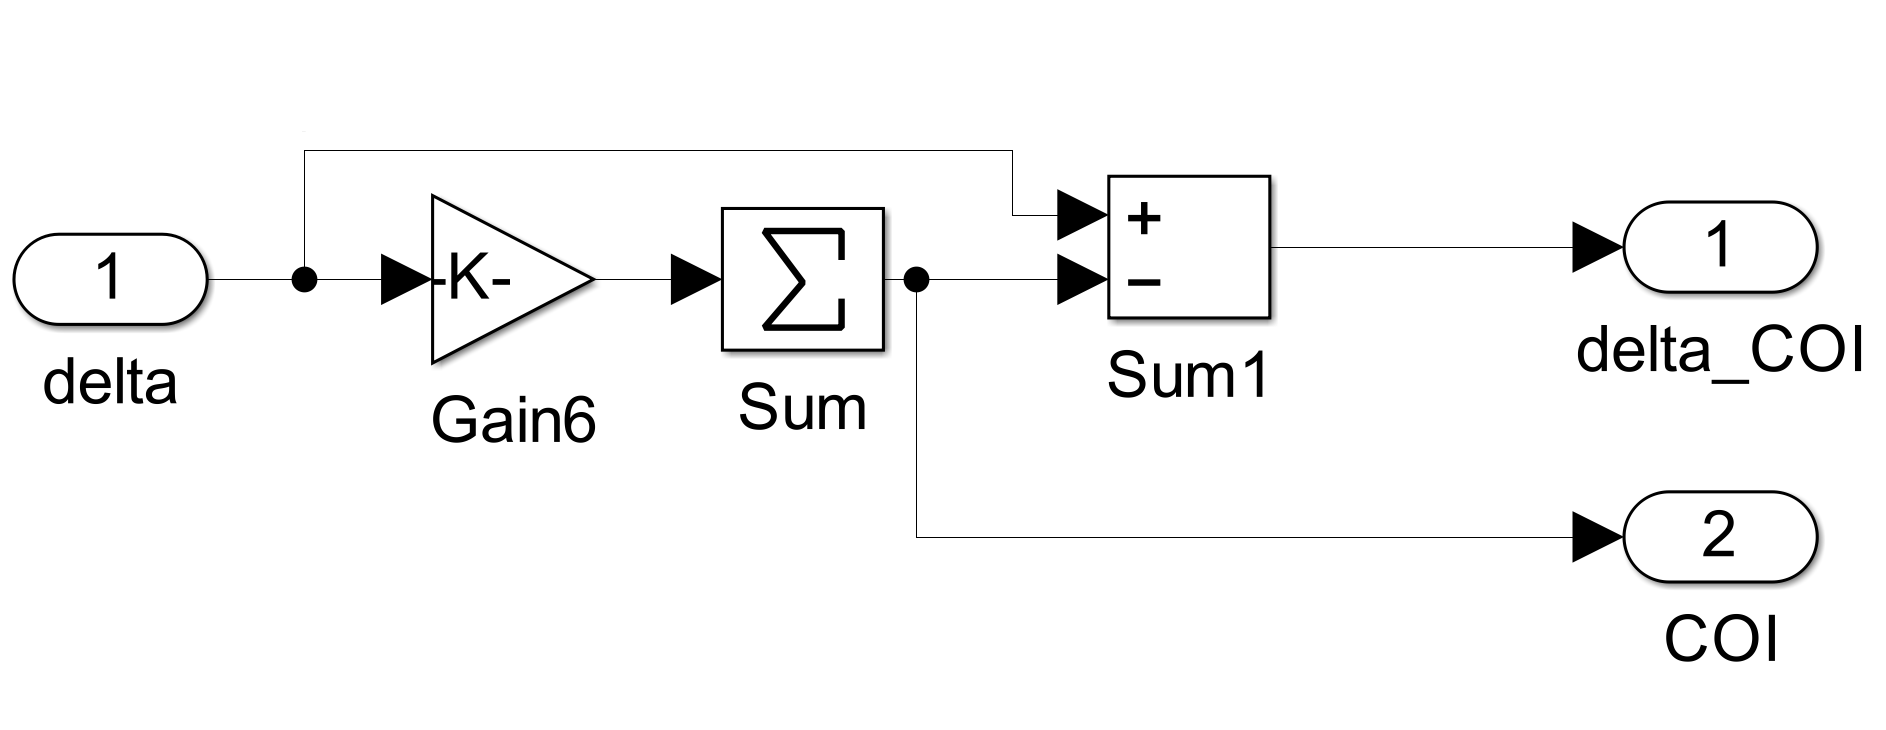
\includegraphics[scale=0.3]{COI Ref}
%		\caption{COI Ref Model}
%		\label{COI Ref}
%		\end{figure}
%		
%		\begin{figure}[H]
%		 \centering
%		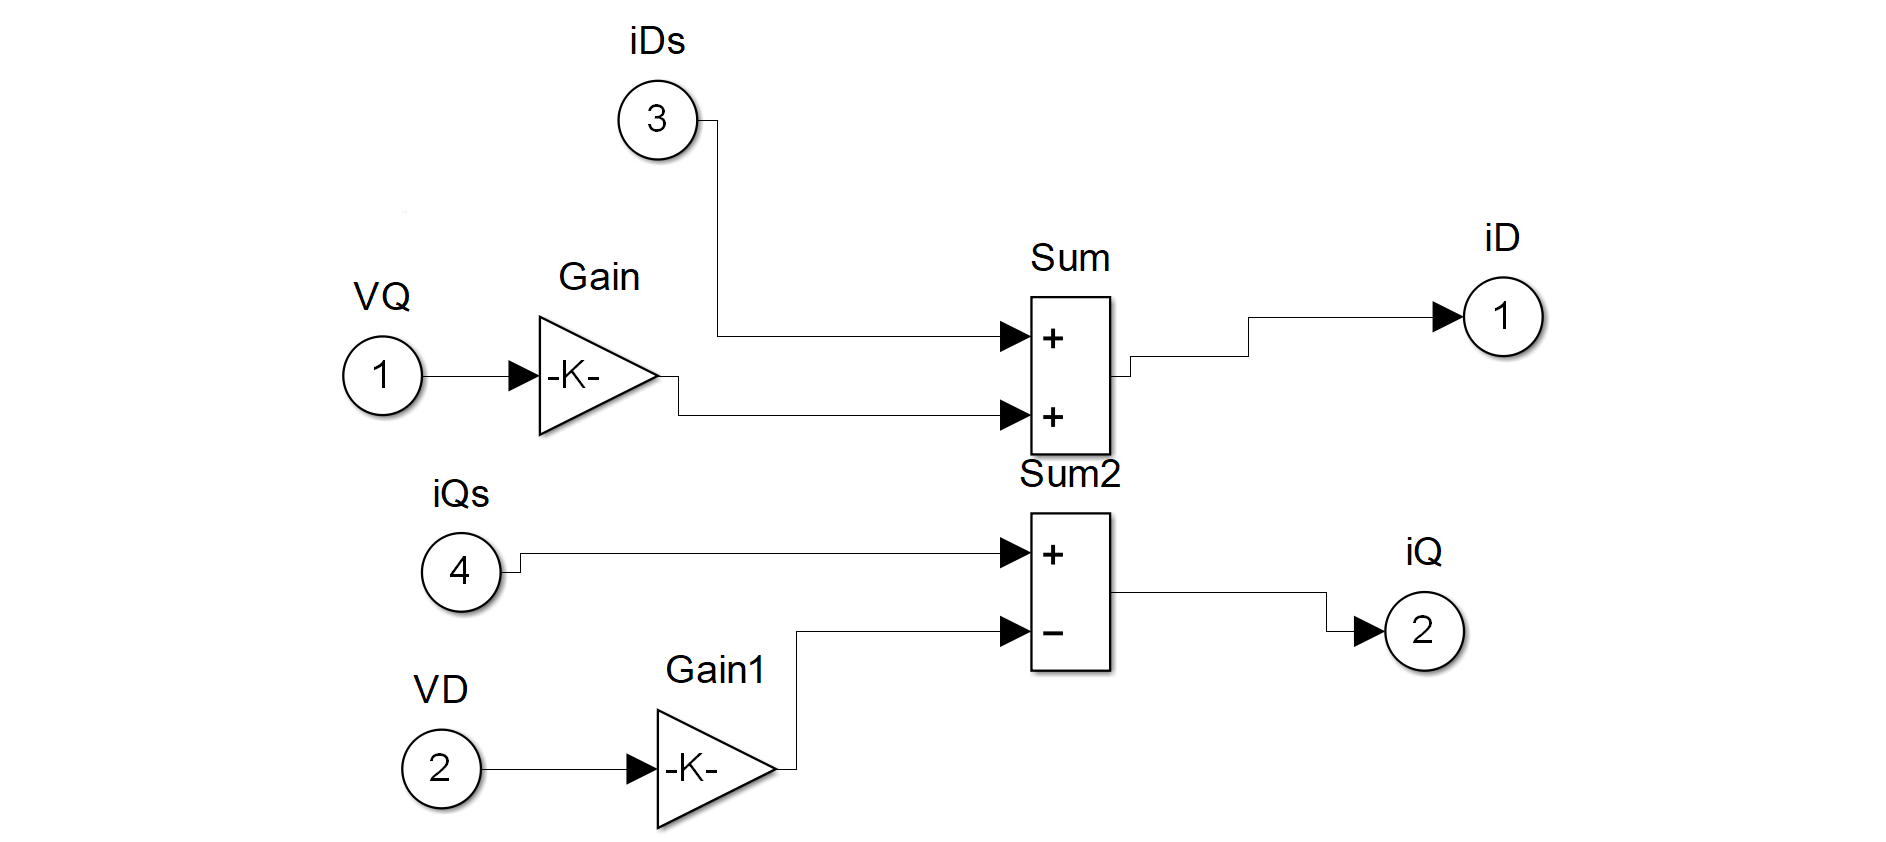
\includegraphics[scale=0.4]{Generator Current}
%		\caption{Generator Currents Model}
%		\label{Generator Current}
%		\end{figure}
		
		\item \textbf{\large Swing Equation Model}: The model shown in Fig. \ref{swing eqn} is for the equation governing the motion of the rotor of a synchronous machine as described previously in Section-2.1 .
		\begin{equation}
		J\frac{d^2\theta_m}{{d(t)}^2}= T_a = T_m - T_e
		\end{equation}
		\begin{figure}[H]
		 \centering
		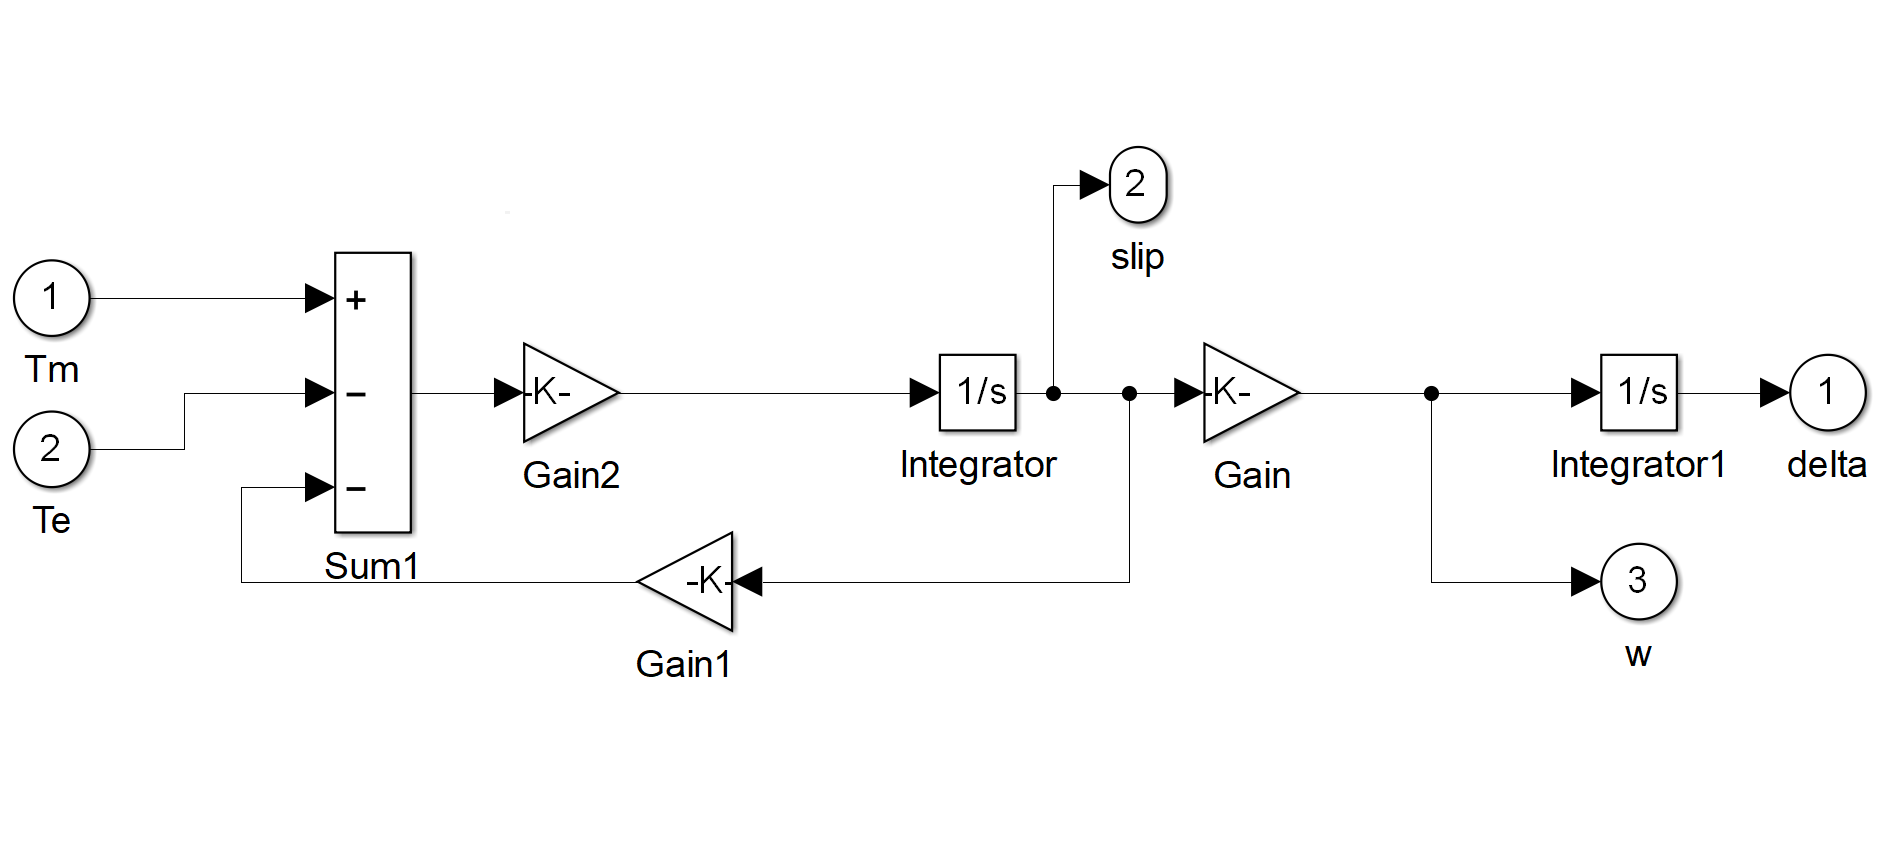
\includegraphics[scale=0.3]{swing eqn}
		\caption{Swing Equation Model}
		\label{swing eqn}
		\end{figure}
		
%		\item \textbf{\large Electric Torque Model}: This is the sub model for creating electric torque from direct axis and quadrature axis current and voltage.
%		\begin{figure}[H]
%		 \centering
%		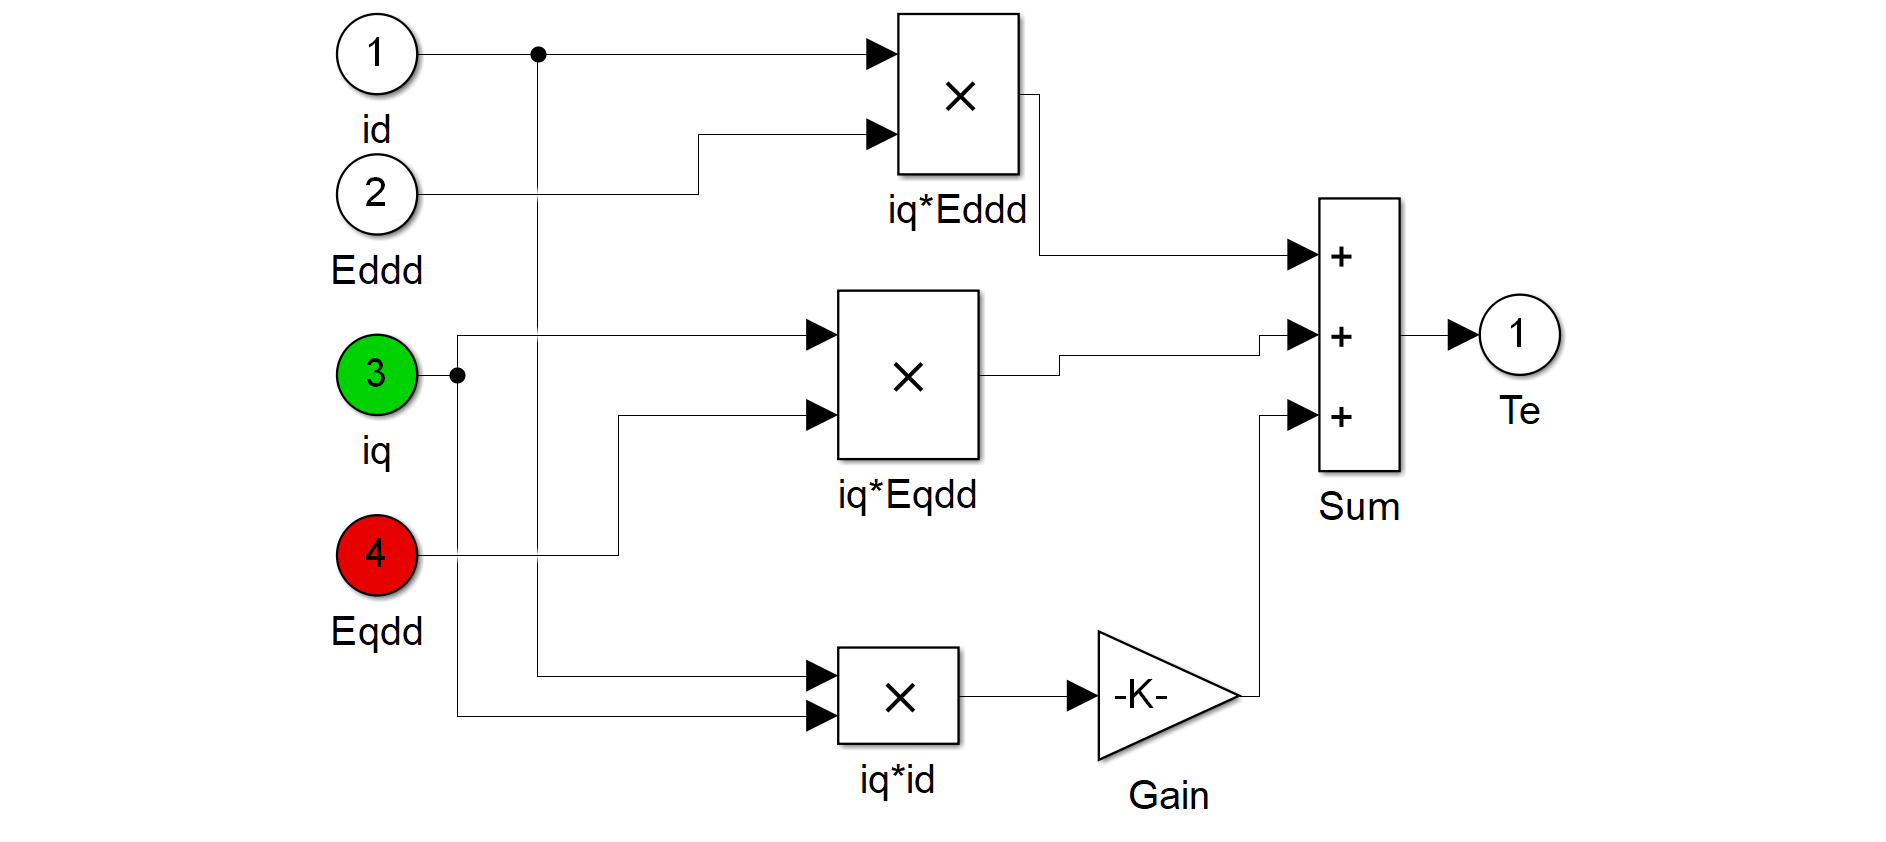
\includegraphics[scale=0.4]{Electric Torque Model}
%		\caption{Electric Torque Model}
%		\label{Electric Torque Model}
%		\end{figure}
%	%	
%	%	\begin{figure}[H]
%	%	 \centering
%	%	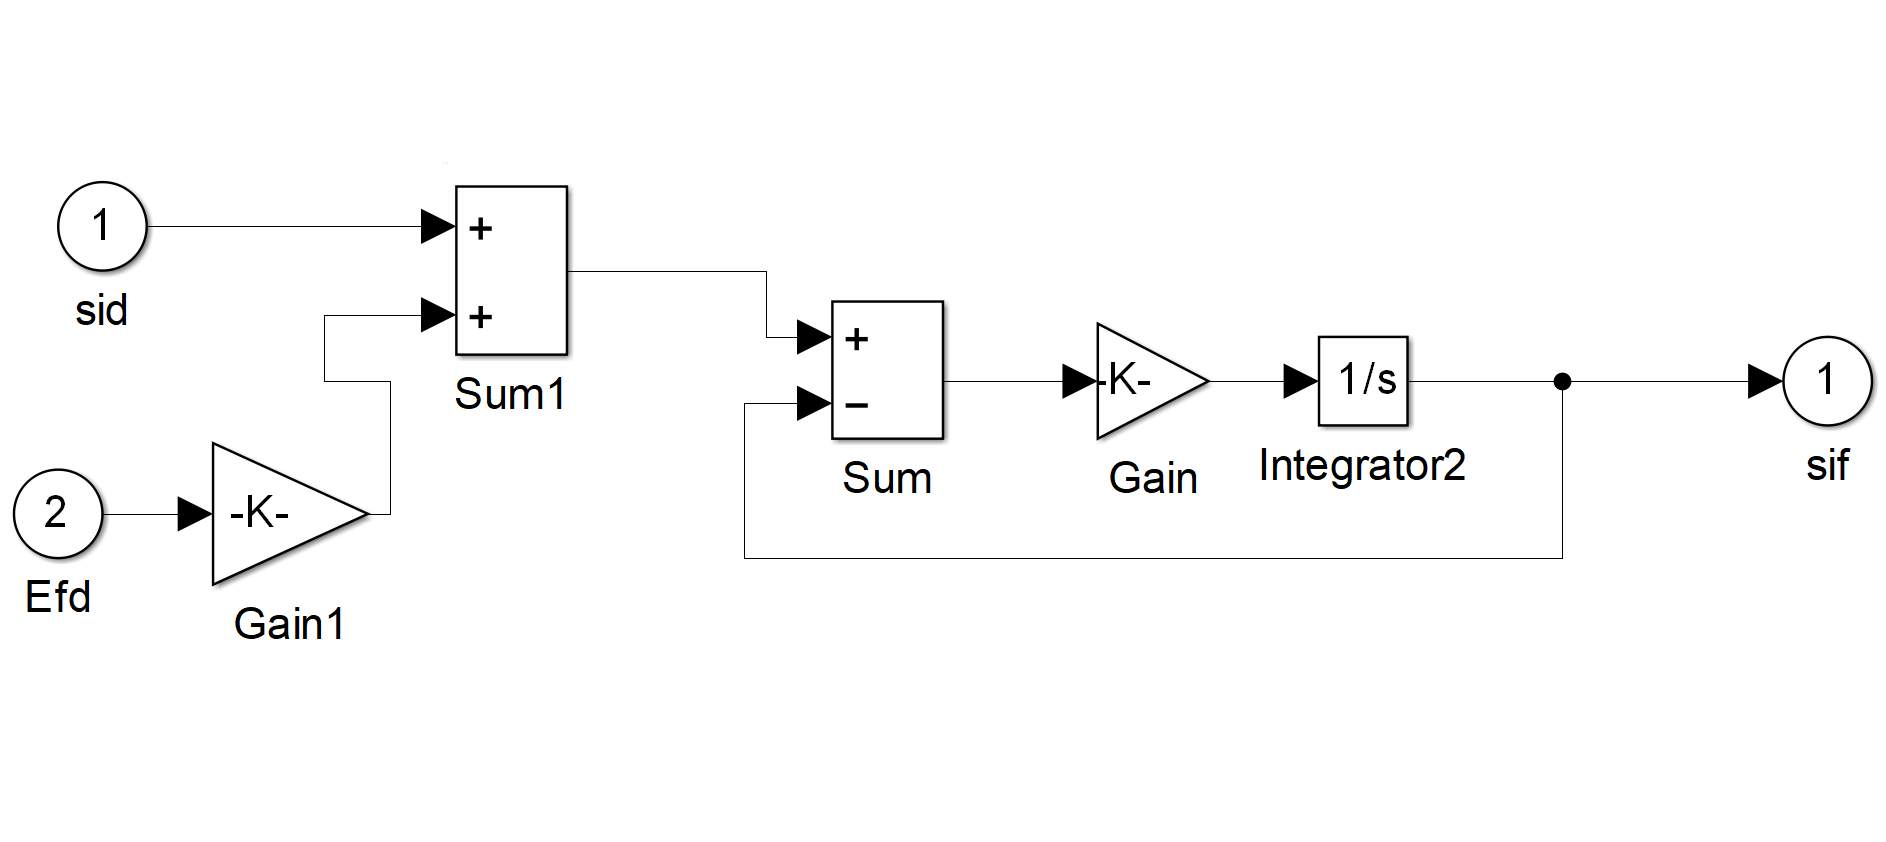
\includegraphics[scale=0.4]{Field Coil}
%	%	\caption{Field Coil}
%	%	\label{Field Coil}
%	%	\end{figure}
	\end{itemize}
%% 2. Turbine System Model =========================================================	
\item \textbf{\large Turbine System Model}: Different Turbine Systems are included such as Speed Governor Hydro Turbine, Speed Governor Reheat Steam turbine and Non Reheat Steam turbine to add Turbine parameters to check system variance in case of real time use.
	
	\begin{figure}[H]
	 \centering
	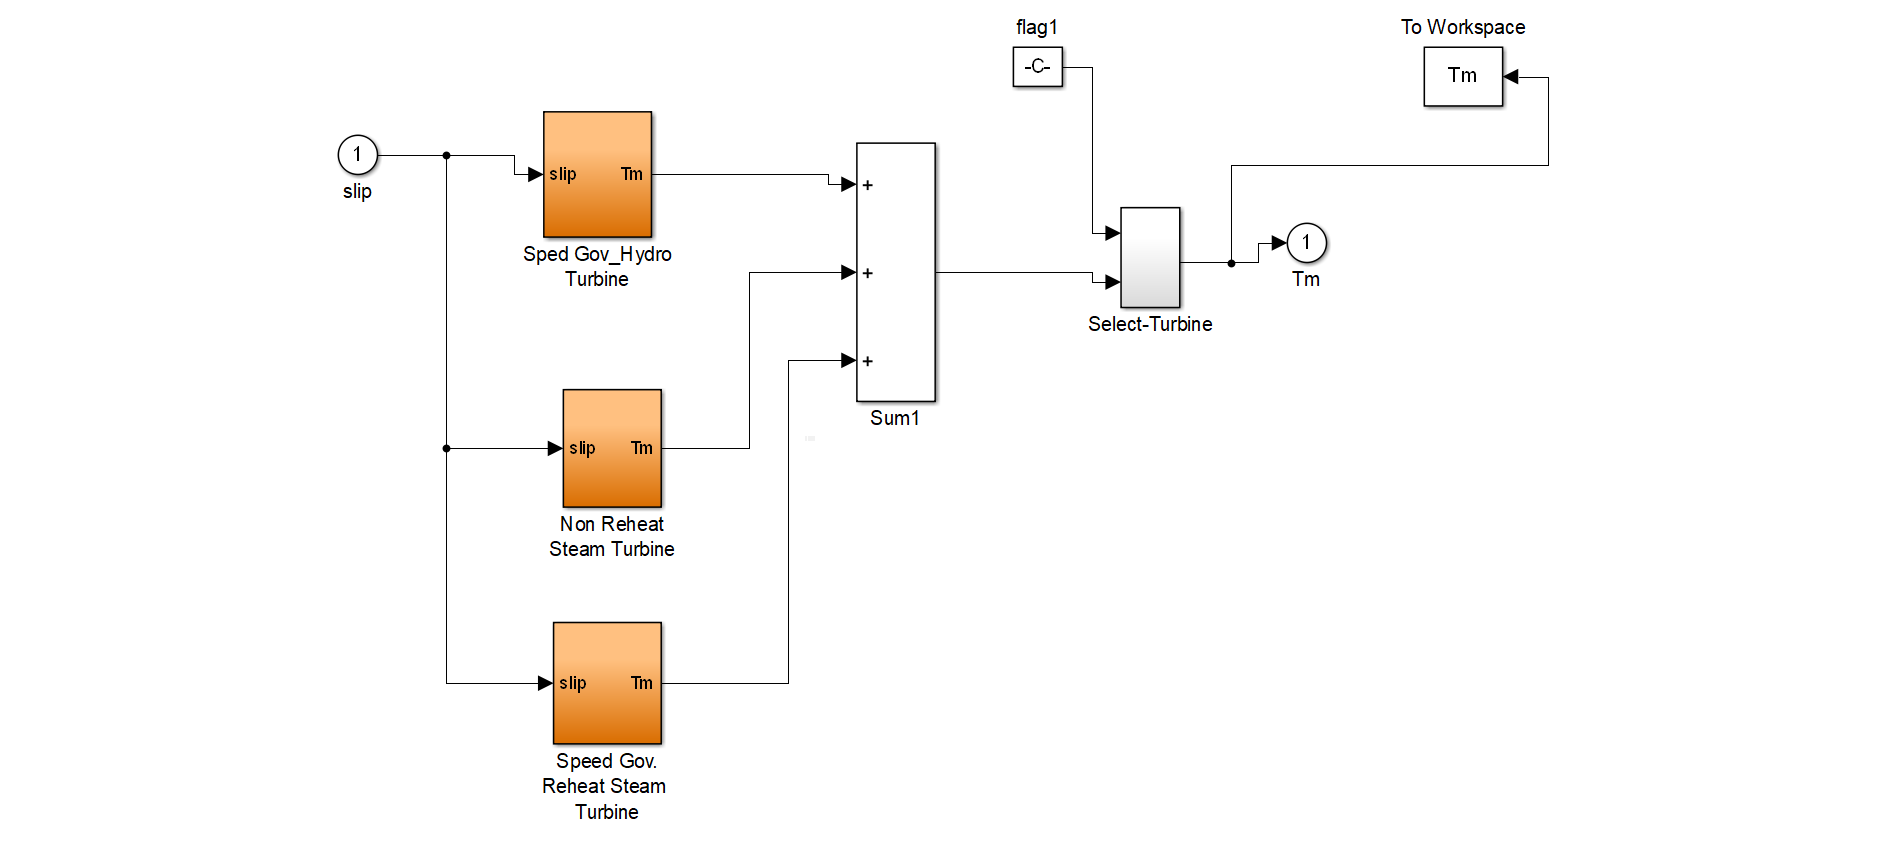
\includegraphics[scale=0.4]{Turbine}
	\caption{Turbine System Model}
	\label{Turbine System Model}
	\end{figure}
	
%	% Turbine System Sub Models-------------------------------------------------
%	\begin{itemize}
%	\item \textbf{\large Turbine System Sub Models}: Three turbine systems are used for a basic generator as follows.
%		\begin{figure}[H]
%		 \centering
%		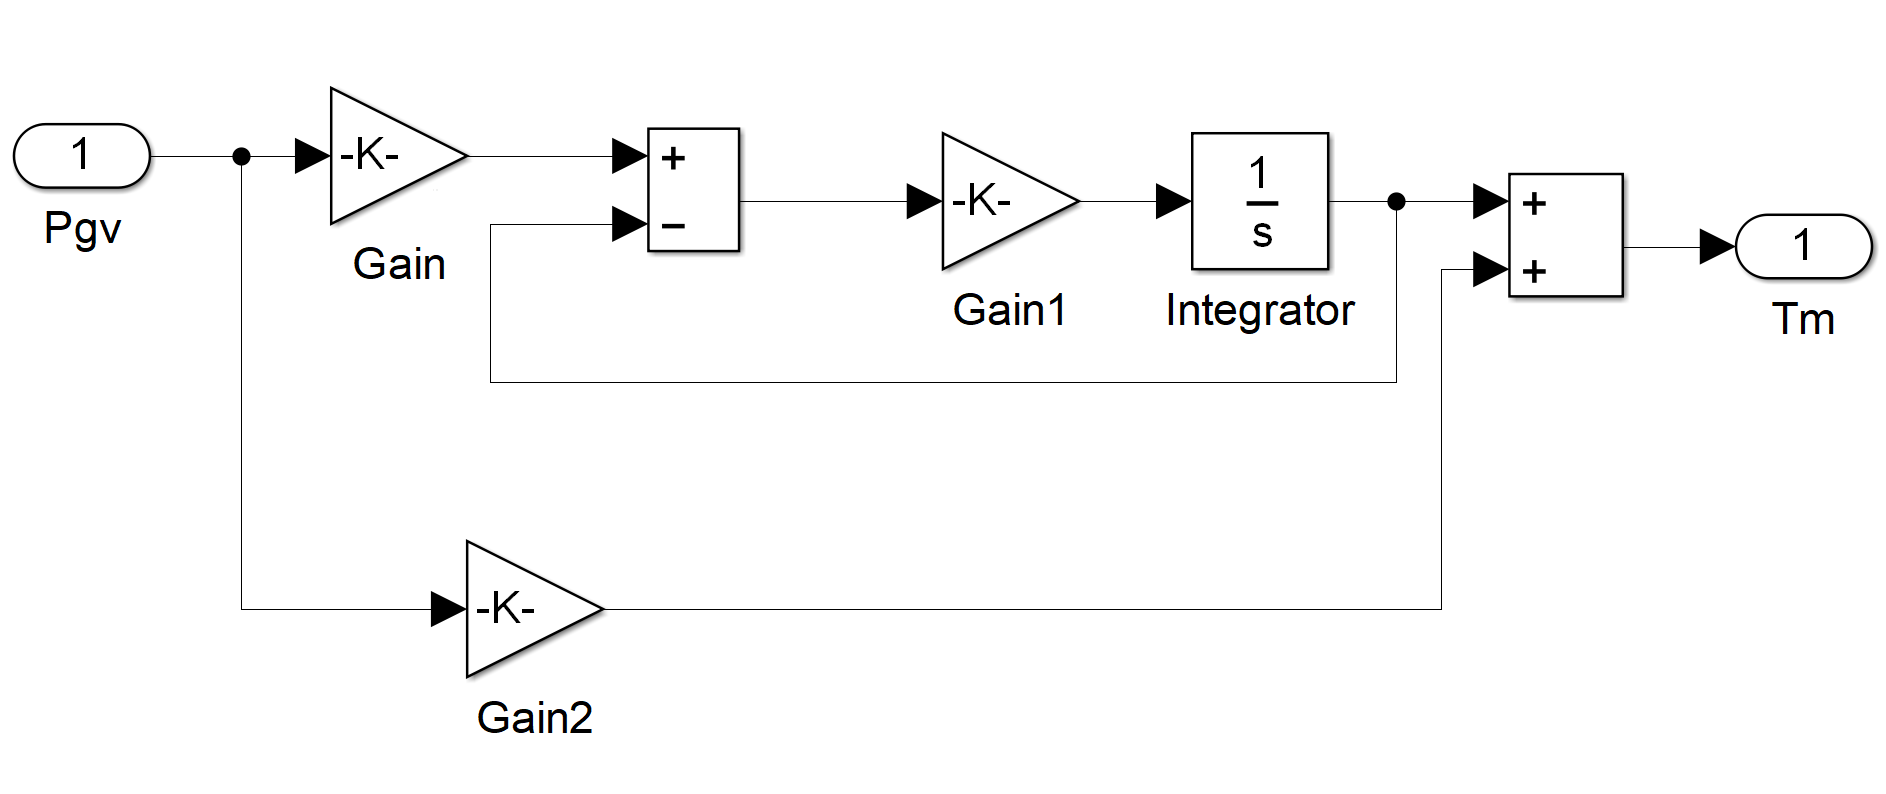
\includegraphics[scale=0.3]{Hydro Turbine Model}
%		\caption{Hydro Turbine Model}
%		\label{Hydro Turbine Model}
%		\end{figure}
%		
%		\begin{figure}[H]
%		 \centering
%		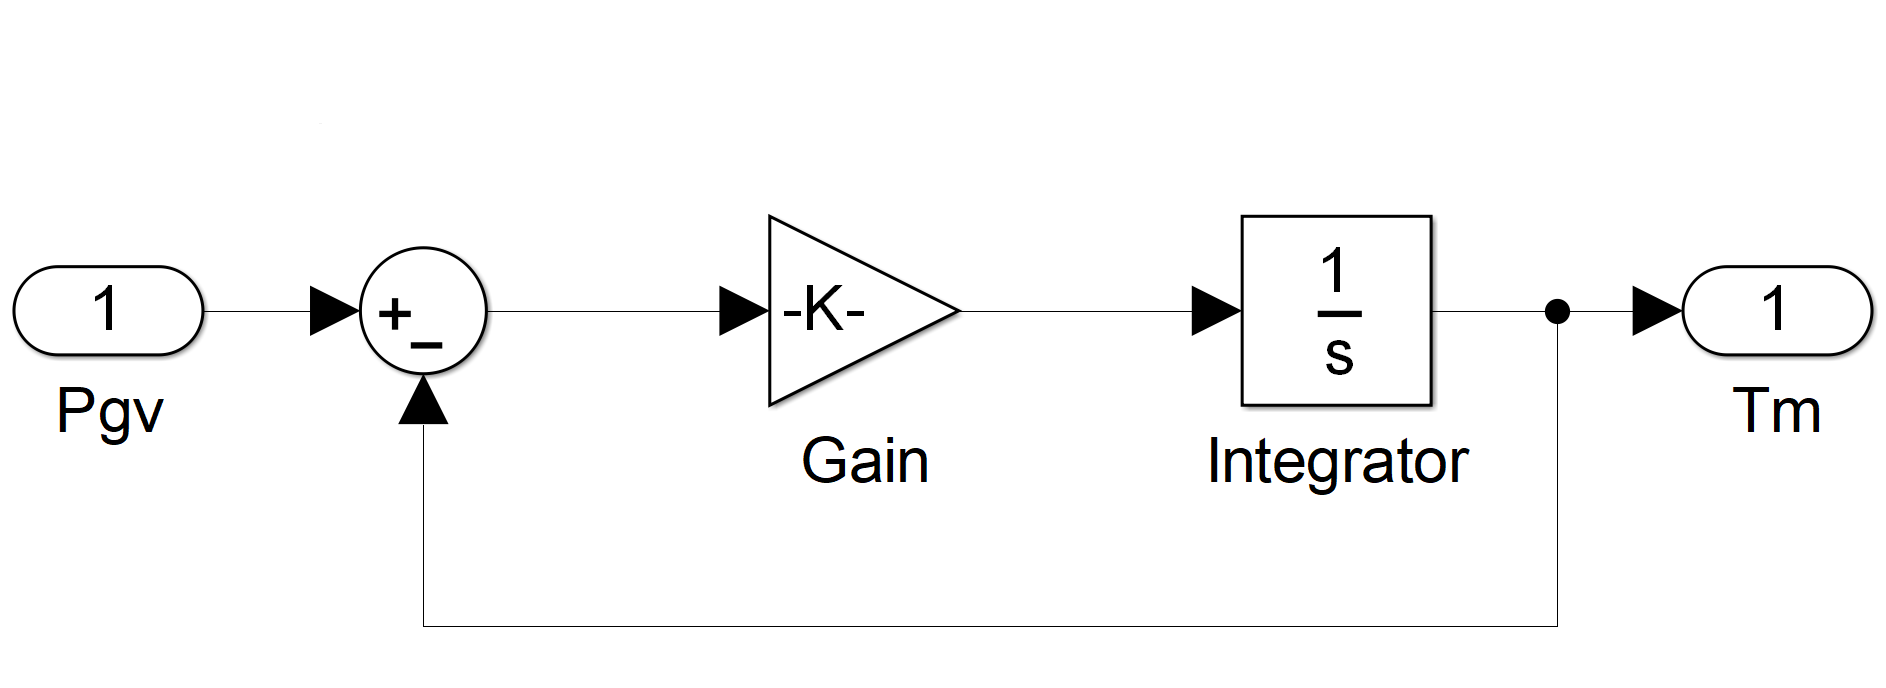
\includegraphics[scale=0.3]{Non Reheat Turbine}
%		\caption{Non Reheat Turbine}
%		\label{Non Reheat Turbine}
%		\end{figure}
%		
%		\begin{figure}[H]
%		 \centering
%		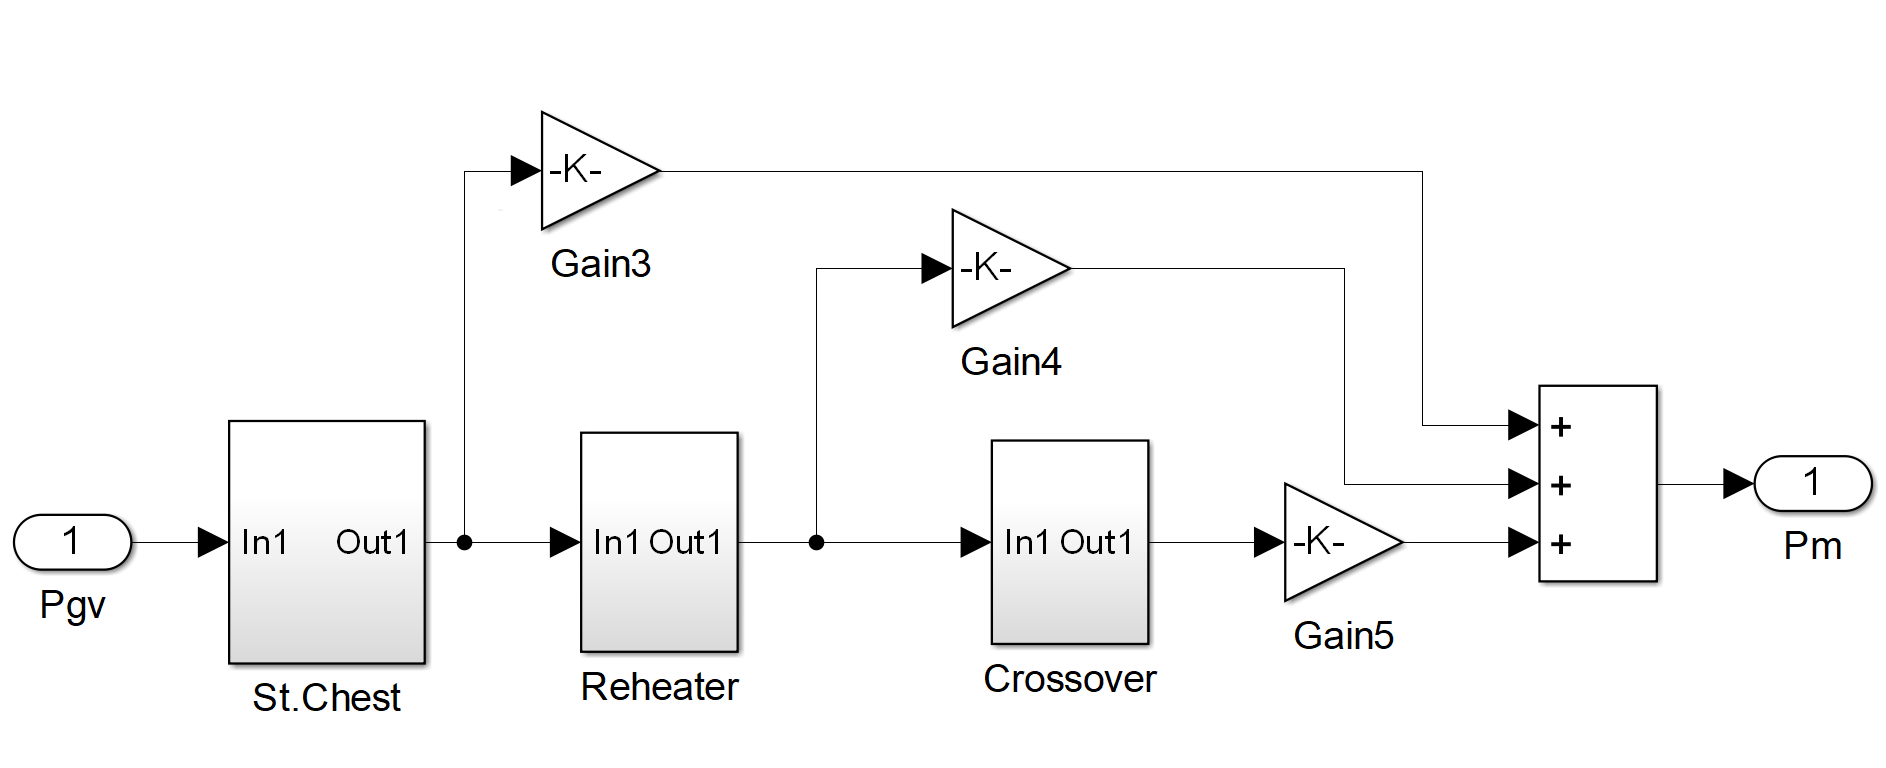
\includegraphics[scale=0.3]{Reheat Turbine}
%		\caption{Reheat Turbine}
%		\label{COI Ref}
%		\end{figure}
%		
%				
%	\item \textbf{\large Turbine Governor System Models}: Turbine governor systems are used for a basic generator as follows.
%		\begin{figure}[H]
%		 \centering
%		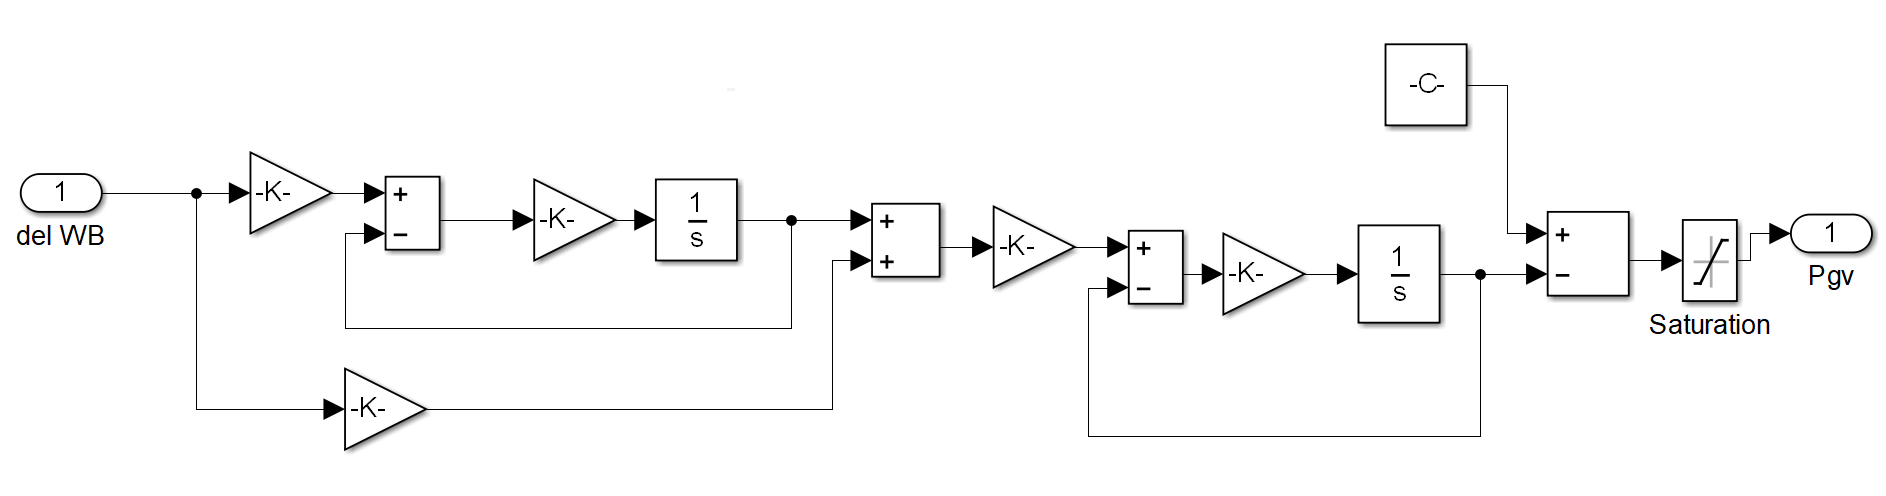
\includegraphics[scale=0.3]{Governor model}
%		\caption{Governor model}
%		\label{Governor model}
%		\end{figure}
%				
%		\begin{figure}[H]
%		 \centering
%		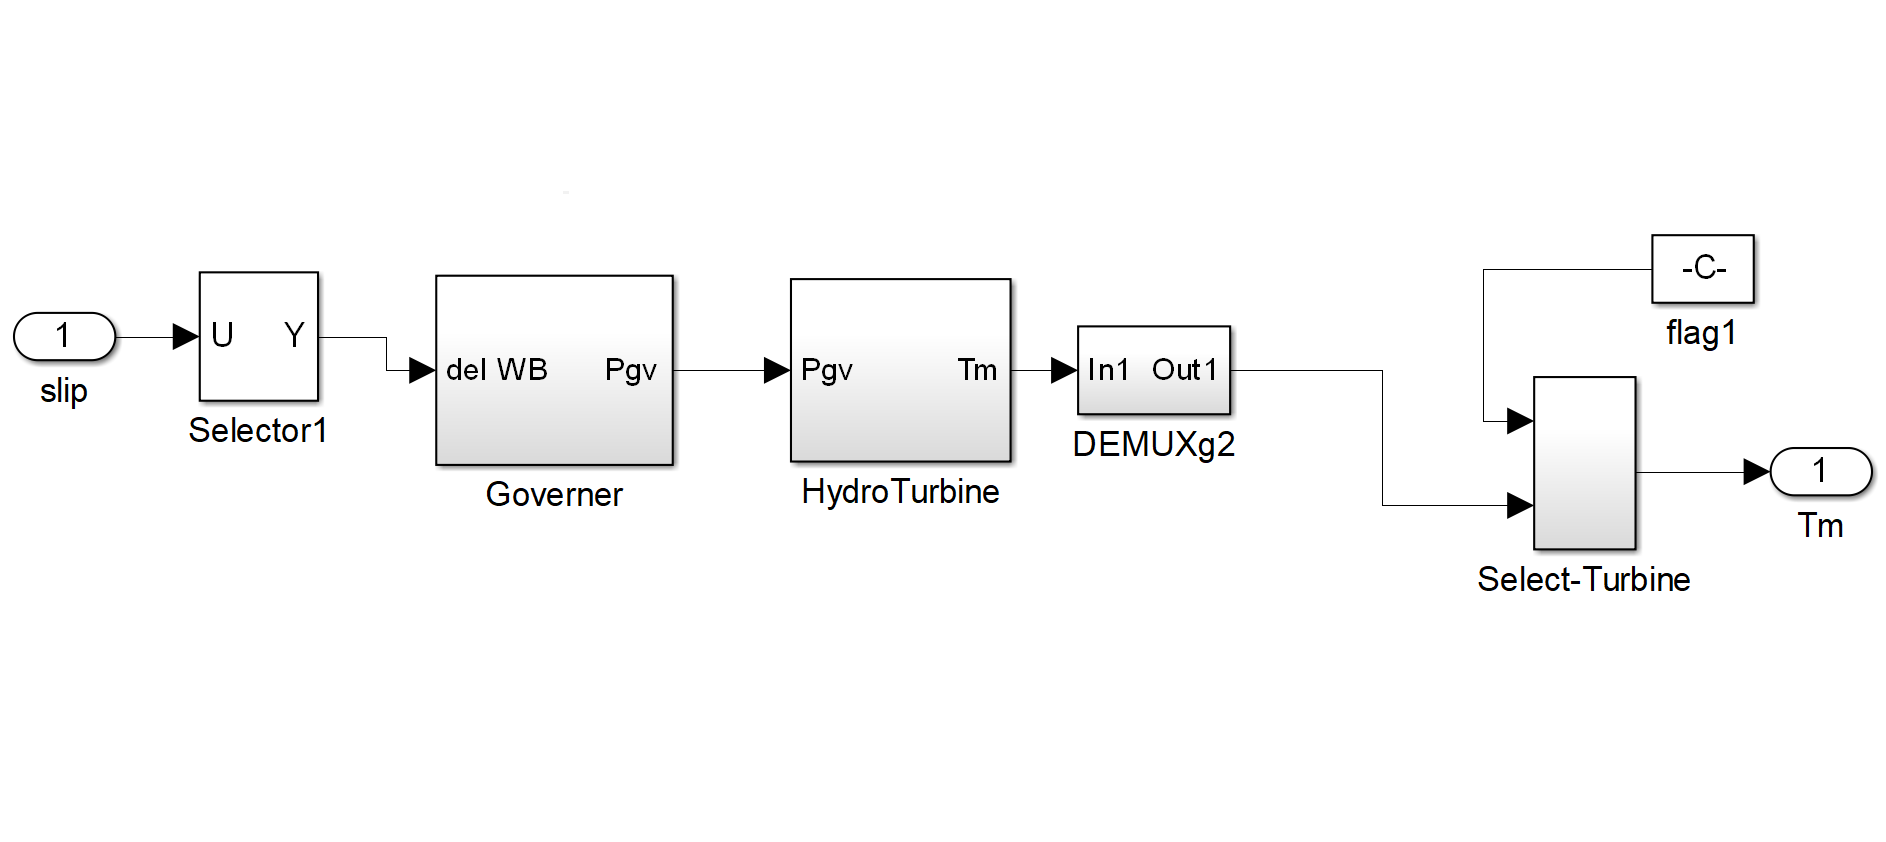
\includegraphics[scale=0.3]{Hydro governer speed turbine}
%		\caption{Hydro Turbine Speed governor}
%		\label{Hydro Turbine Speed governor}
%		\end{figure}
%		
%		\begin{figure}[H]
%		 \centering
%		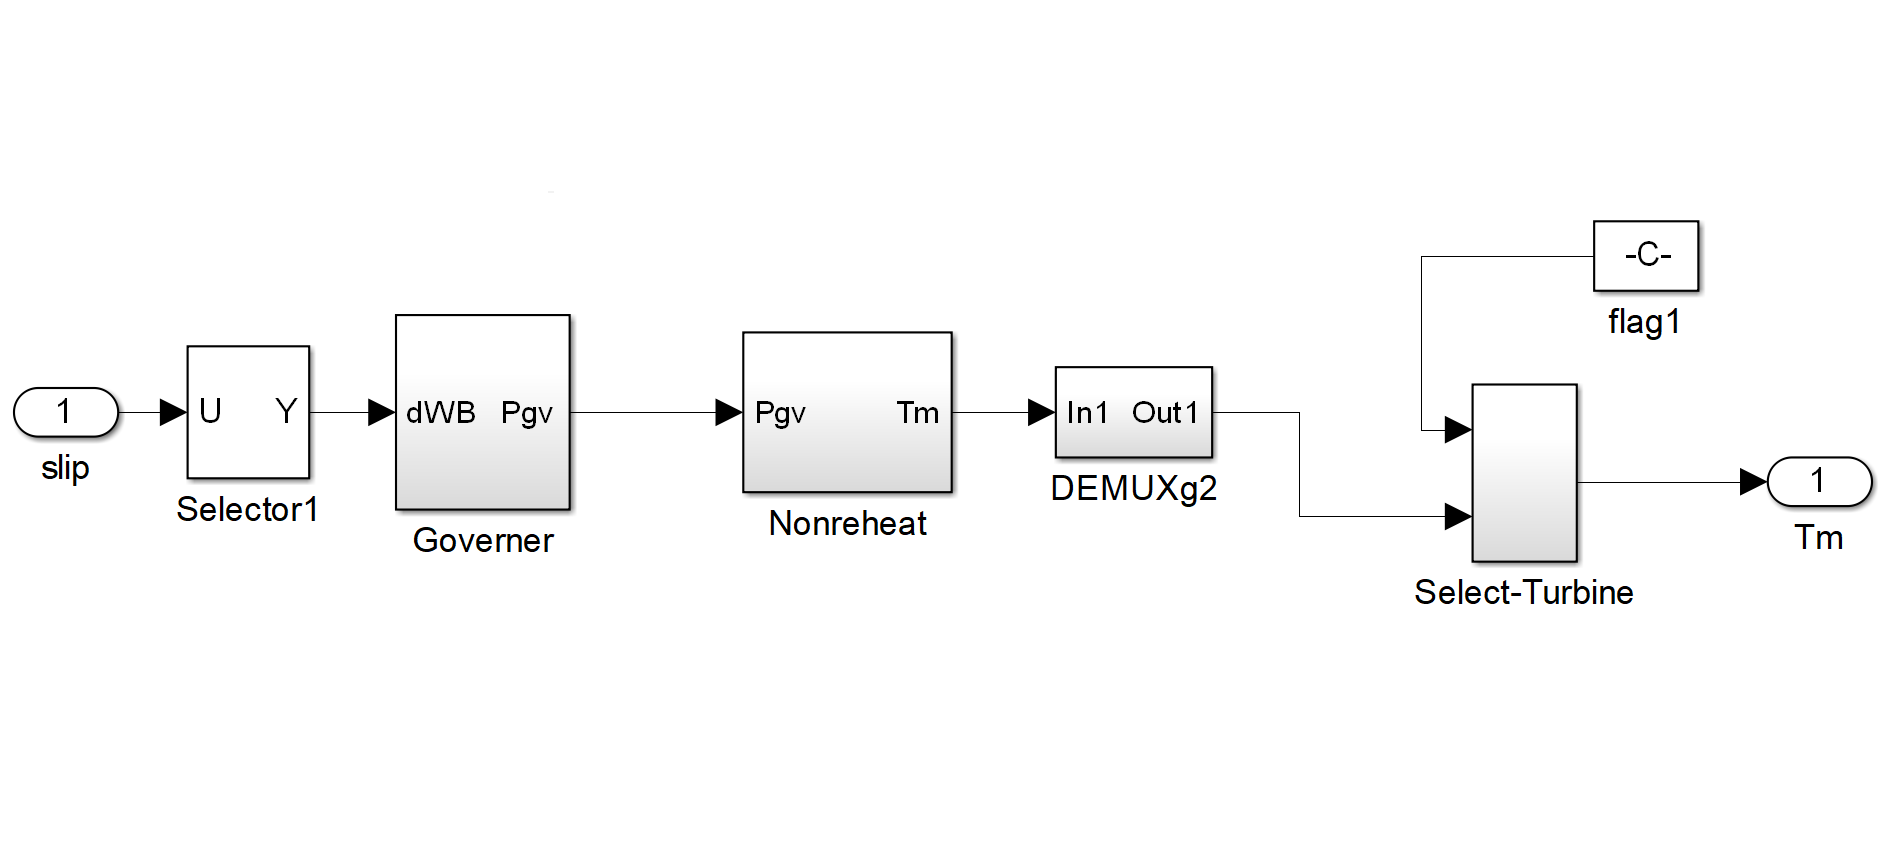
\includegraphics[scale=0.3]{Non Reheat Speed Turbine}
%		\caption{Non Reheat Turbine Speed Governor}
%		\label{Non Reheat Turbine Speed Governor}
%		\end{figure}
%		
%		\begin{figure}[H]
%		 \centering
%		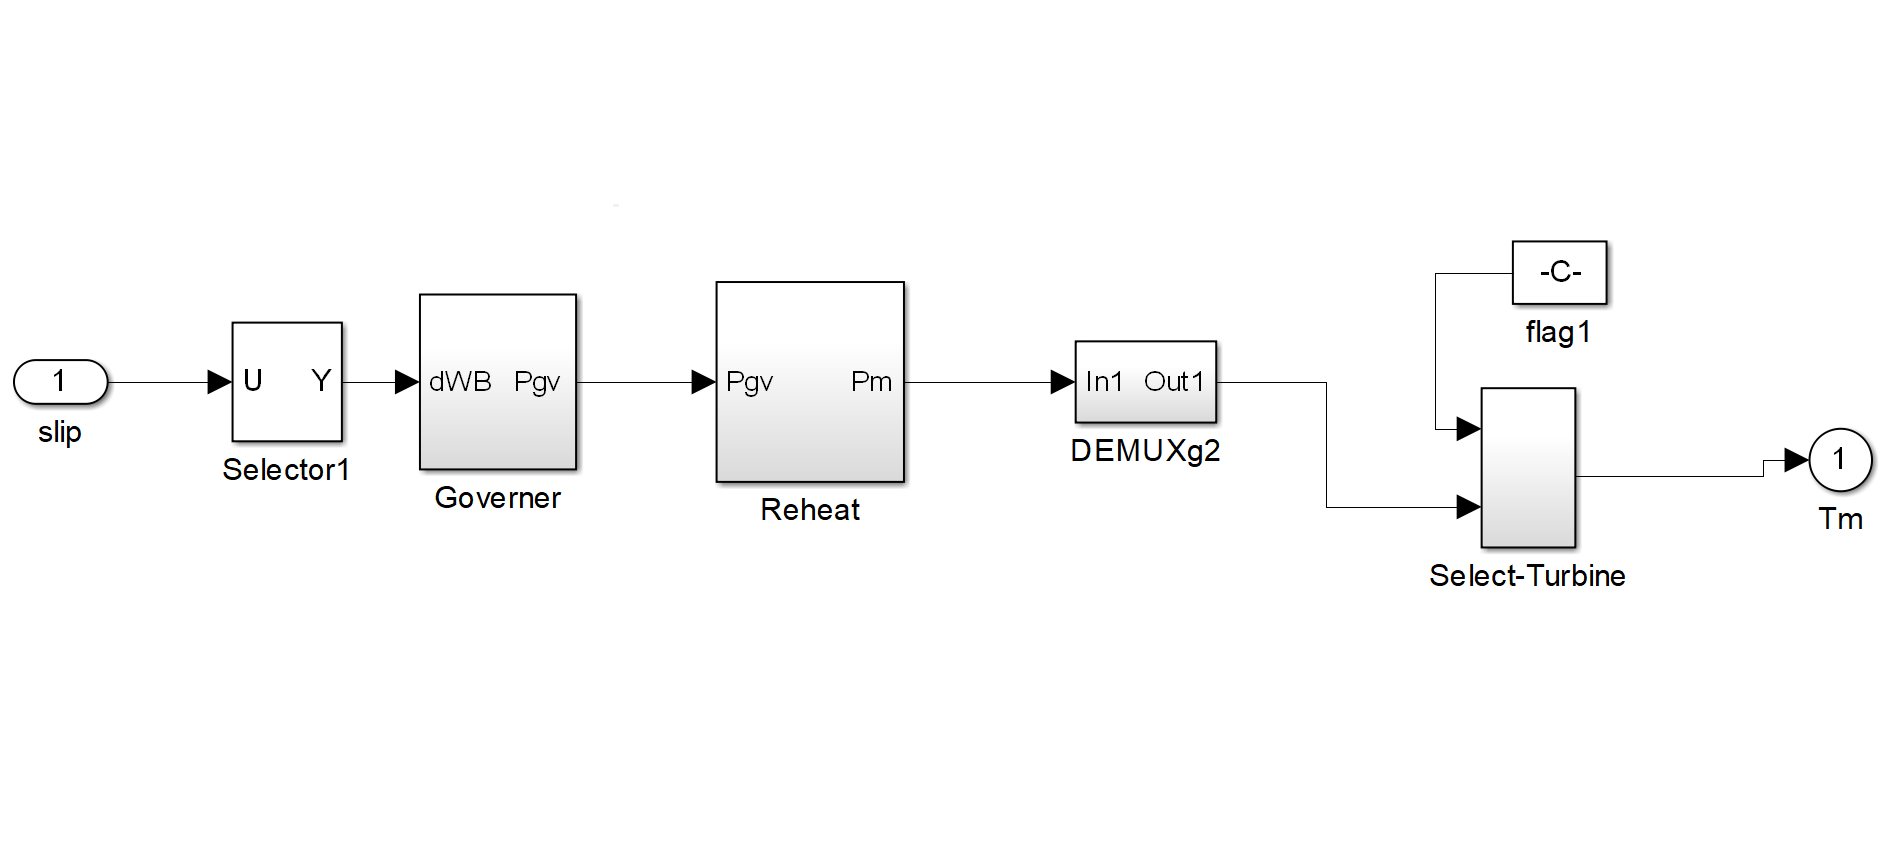
\includegraphics[scale=0.3]{Reheat Speed turbine Governor}
%		\caption{Reheat Turbine Speed Governor}
%		\label{Reheat Turbine Speed Governor}
%		\end{figure}
%	\end{itemize}
	
%% 3. Excitation System Model===================================================	
\item \textbf{\large Excitation System Model}: This is an excitation system created to do the work of an generator exciter, it takes input of Vg, Vs, IFD and Ig and with the help of different exciter system it  produces the Excitation voltage(EFD) and passes to the generator.
	
	\begin{figure}[H]
	 \centering
	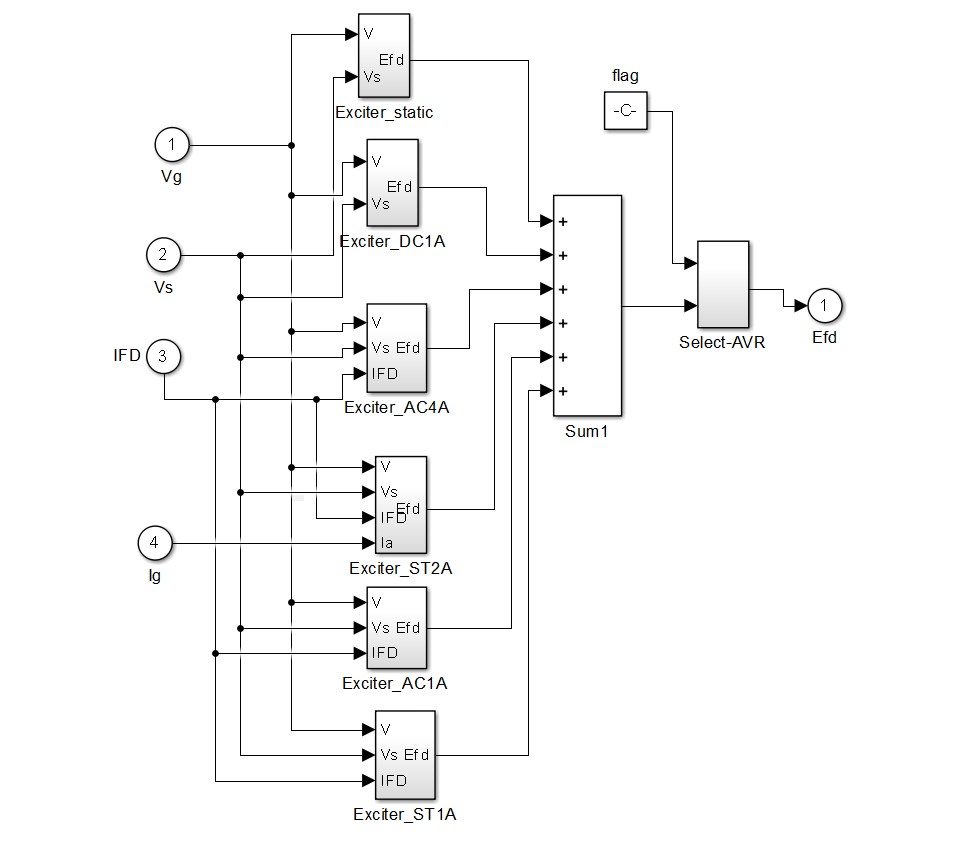
\includegraphics[scale=0.5]{Excitation Model}
	\caption{Excitation Model}
	\label{Excitation Model}
	\end{figure}
	
%	% Excitation System Sub Models-------------------------------------------------
%	\begin{itemize}
%	\item \textbf{\large Excitation System Sub Models}: Taking different inputs as stated in previous slide the different excitation sub part models are created to prepare whole Excitation System Model. The sum of these sub exciter models make a complete excitation system.
%		\begin{figure}[H]
%		 \centering
%		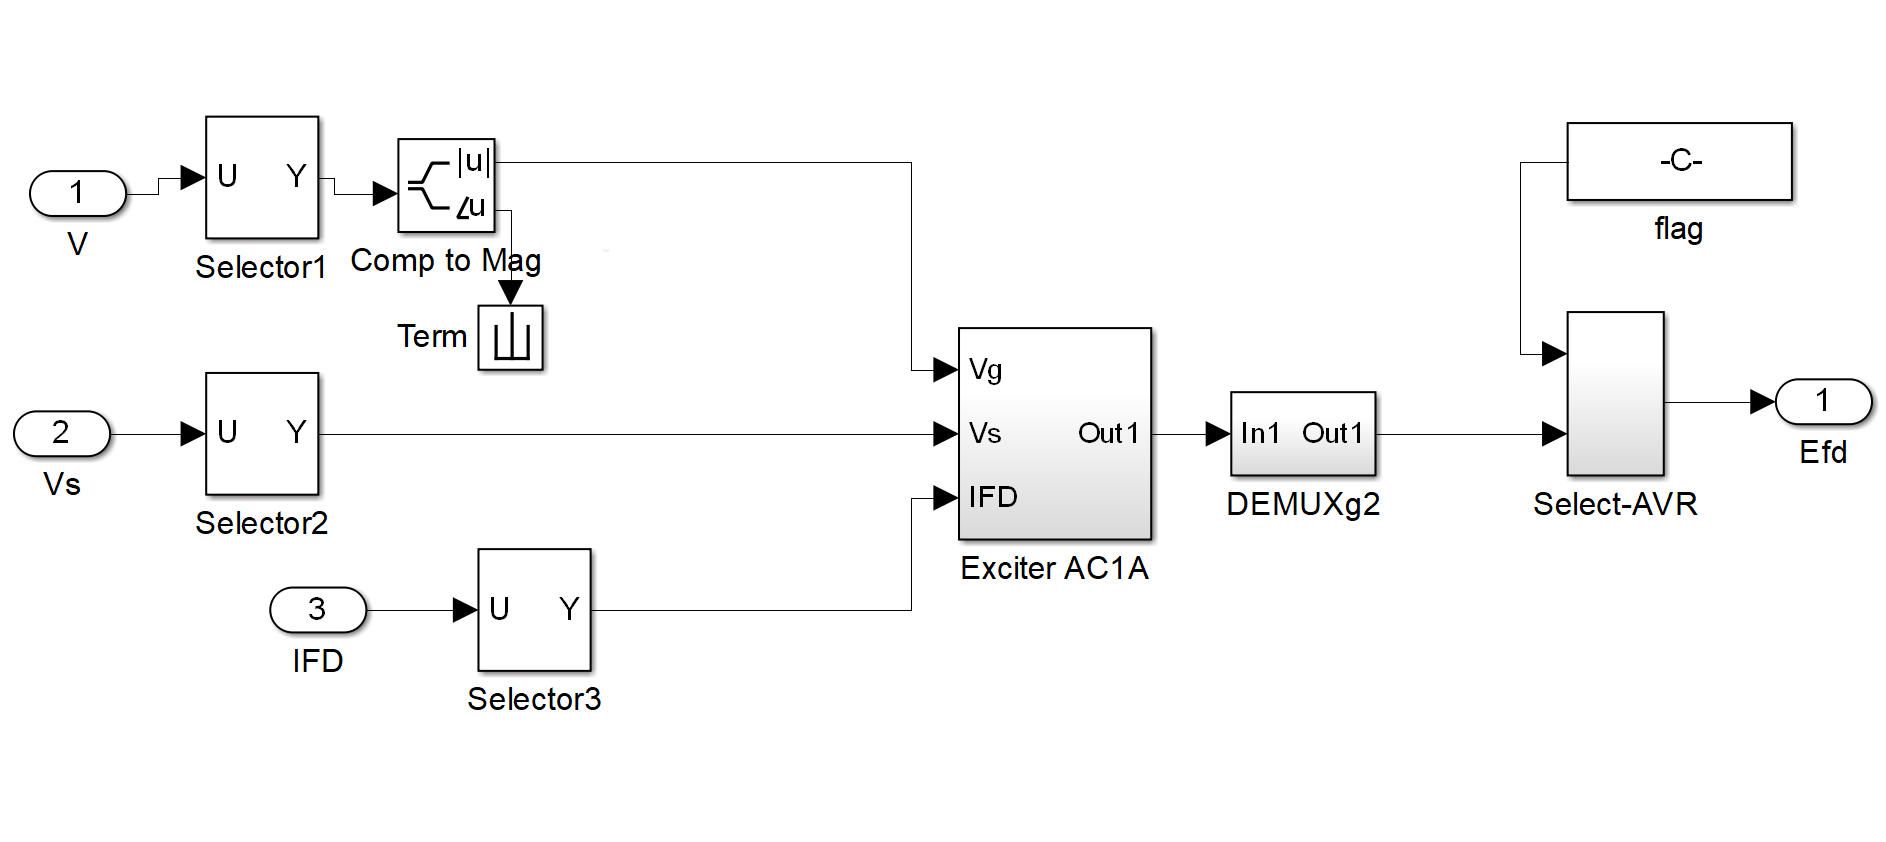
\includegraphics[scale=0.3]{Exciter AC1A}
%		\caption{Exciter AC1A}
%		\label{Exciter AC1A}
%		\end{figure}
%		
%		\begin{figure}[H]
%		 \centering
%		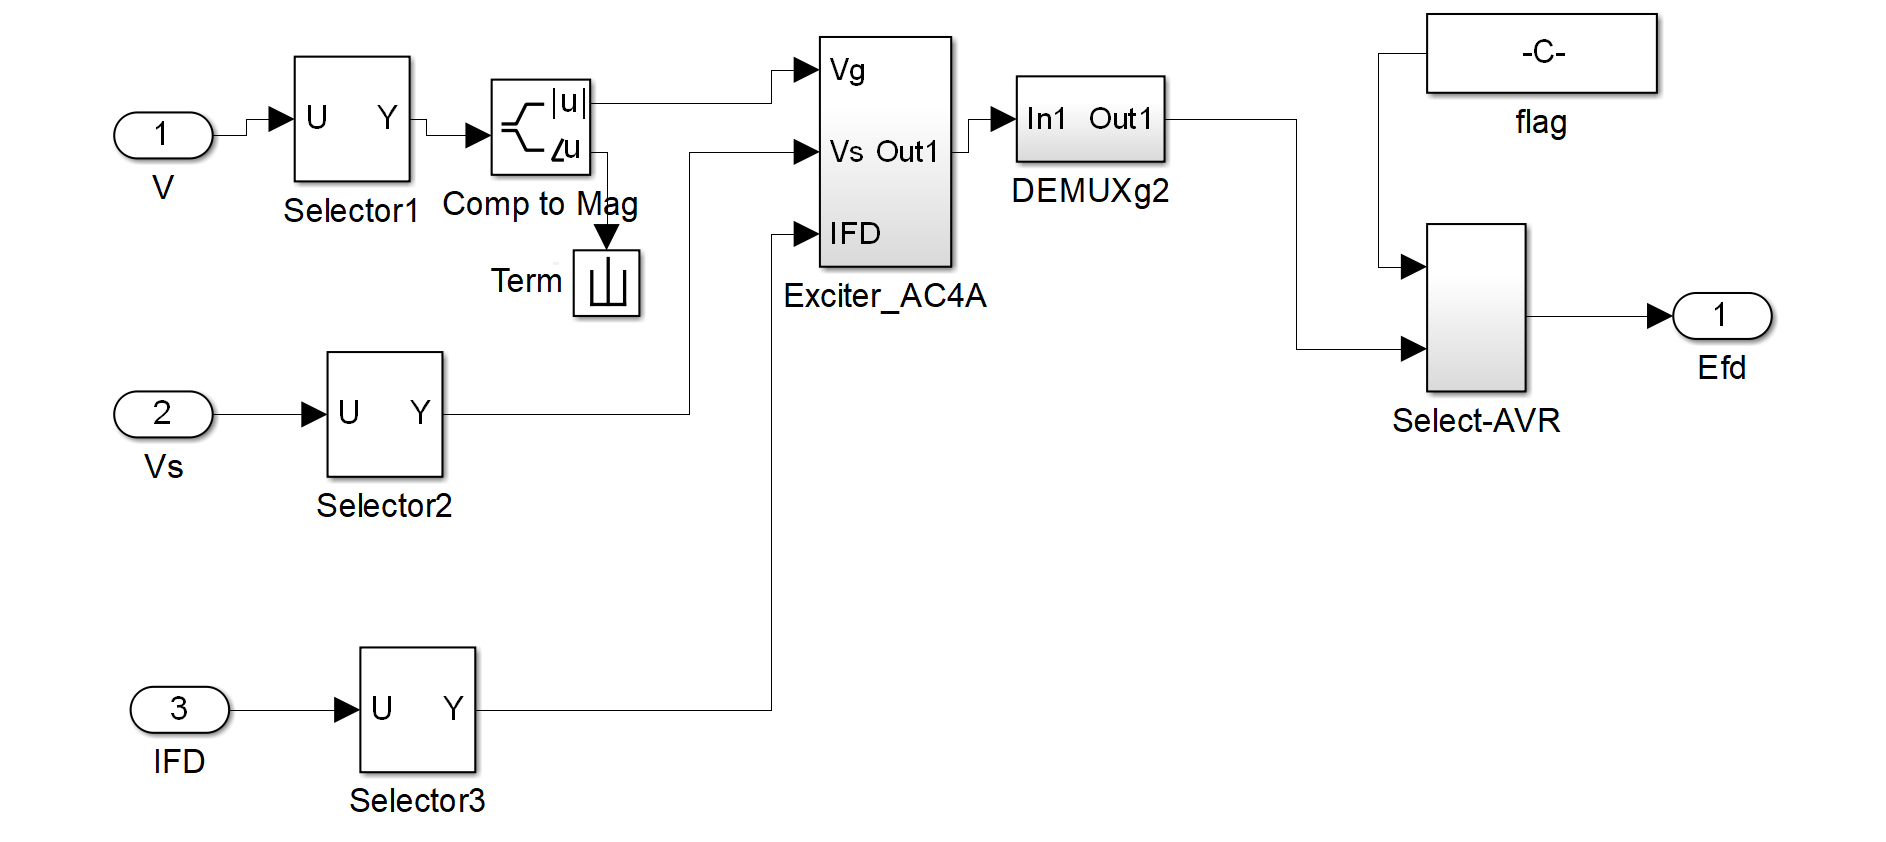
\includegraphics[scale=0.3]{Exciter AC4A}
%		\caption{Exciter AC4A}
%		\label{Exciter AC4A}
%		\end{figure}
%		
%		\begin{figure}[H]
%		 \centering
%		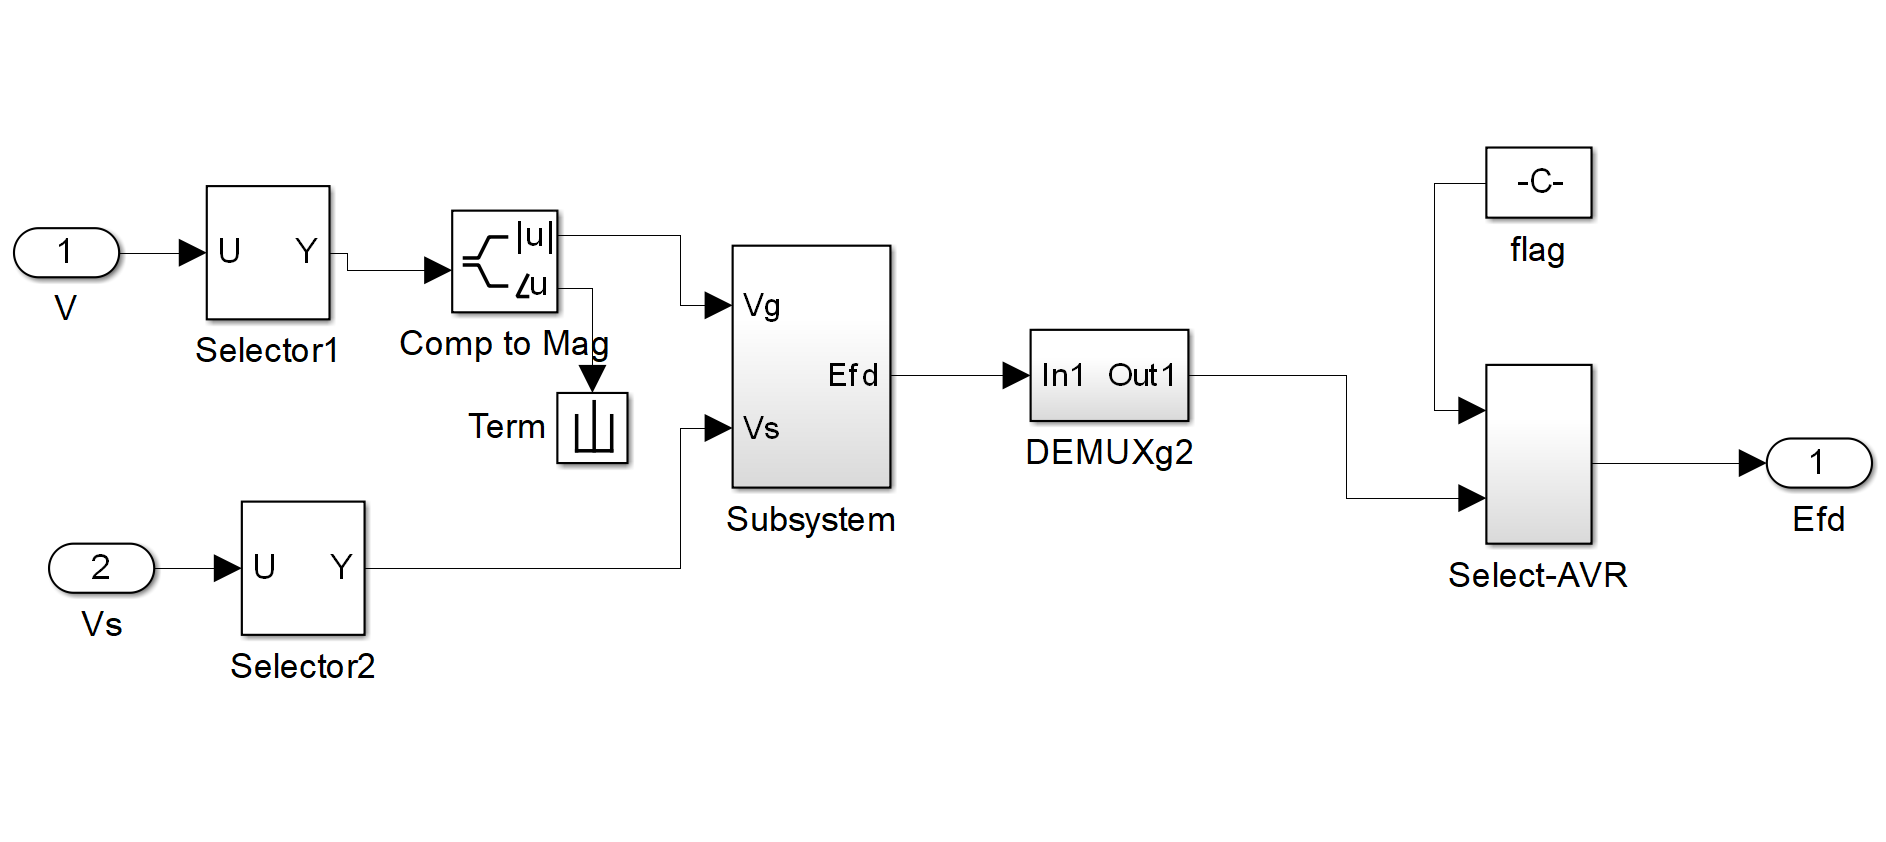
\includegraphics[scale=0.3]{Exciter DC1A}
%		\caption{Exciter DC1A}
%		\label{Exciter DC1A}
%		\end{figure}
%		
%		\begin{figure}[H]
%		 \centering
%		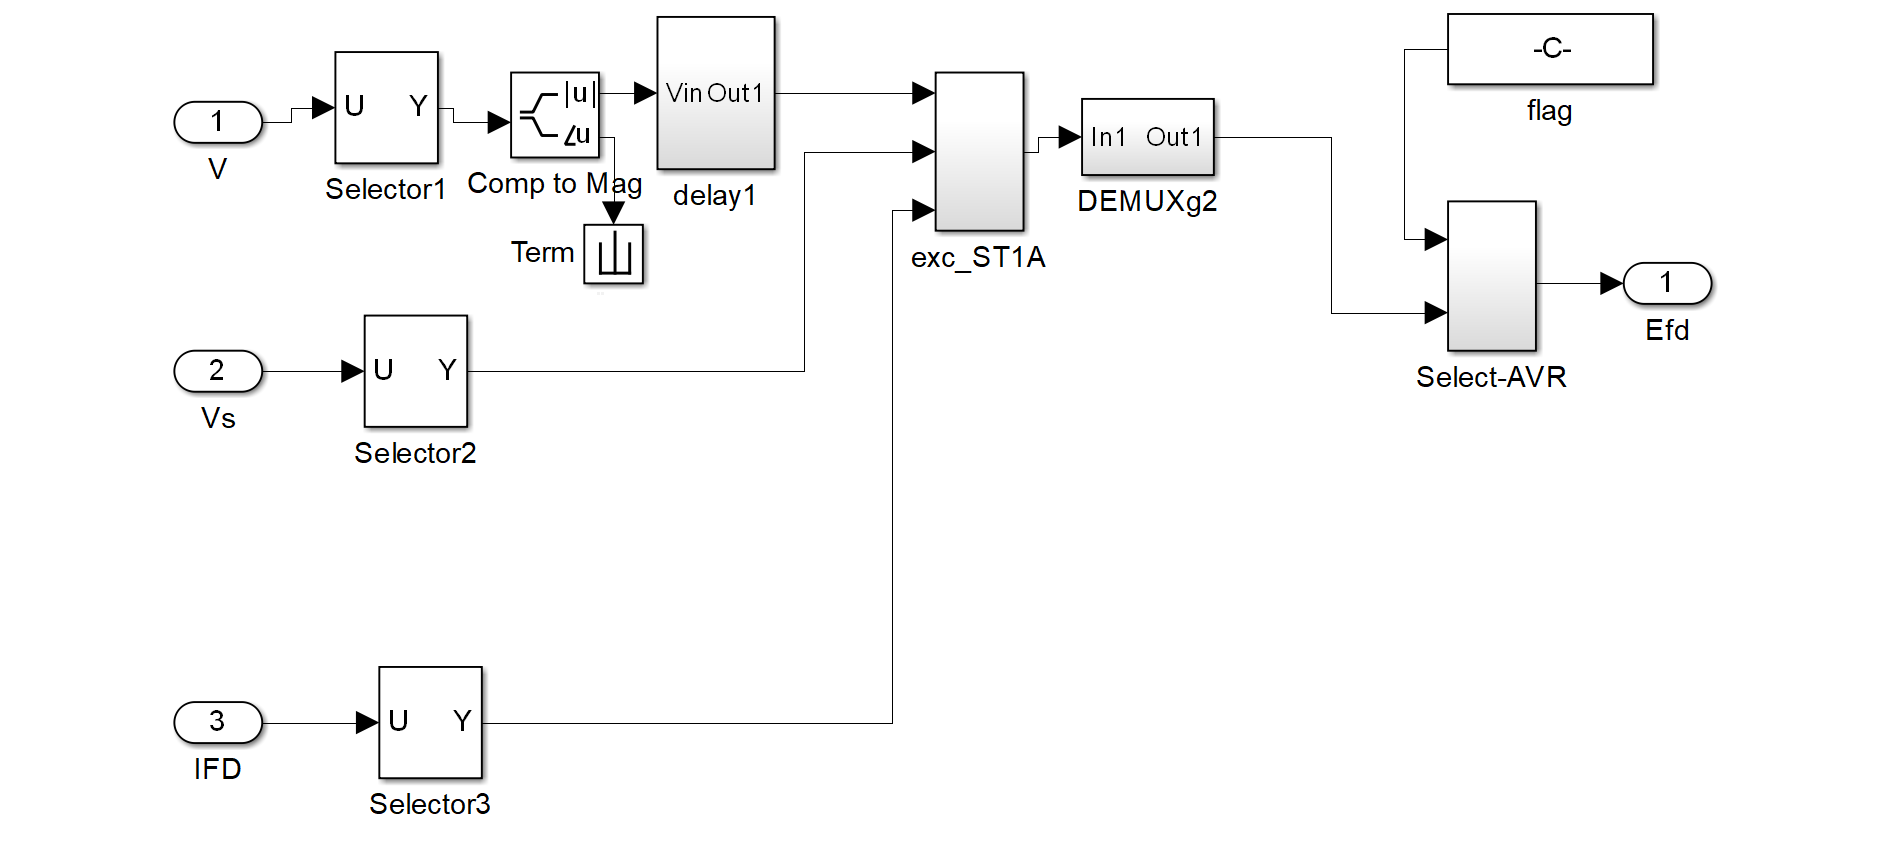
\includegraphics[scale=0.3]{Exciter ST1A}
%		\caption{Exciter ST1A}
%		\label{Exciter ST1A}
%		\end{figure}
%		
%		\begin{figure}[H]
%		 \centering
%		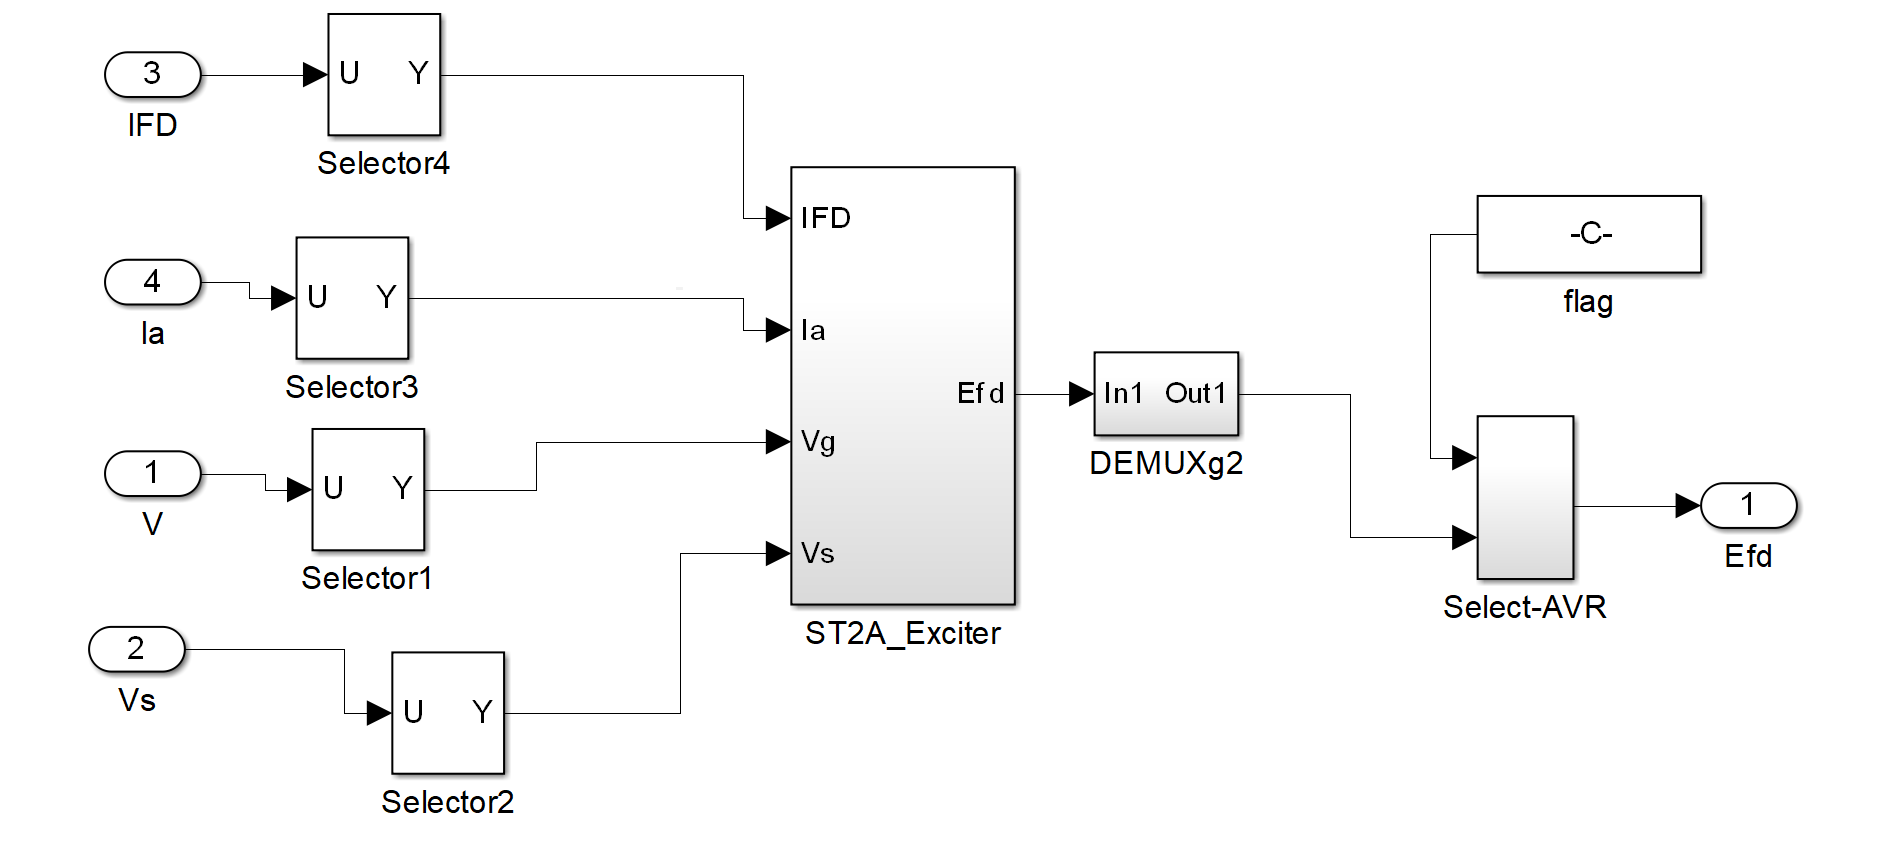
\includegraphics[scale=0.3]{Exciter ST4A}
%		\caption{Exciter ST4A}
%		\label{Exciter ST4A}
%		\end{figure}
%		
%		\begin{figure}[H]
%		 \centering
%		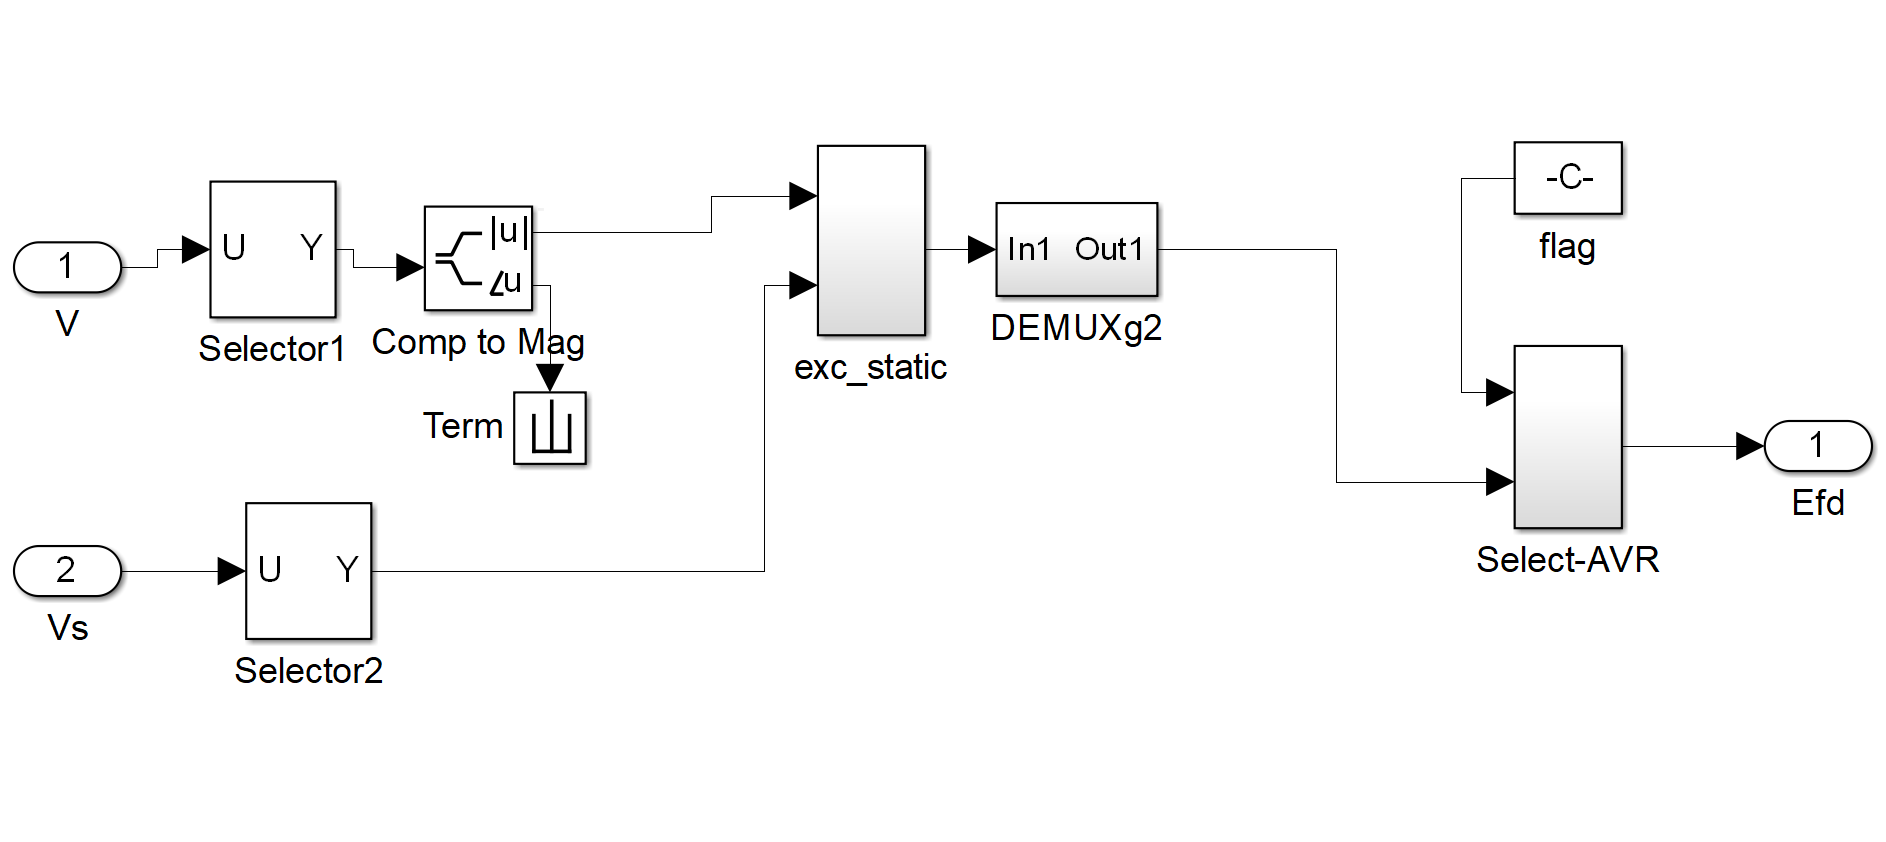
\includegraphics[scale=0.3]{Static Excitor System}
%		\caption{Static Exciter System}
%		\label{Static Exciter System}
%		\end{figure}
%				
%	\end{itemize}

%% 4. Static Loads Model===================================================	
\item \textbf{\large Static Load Model}: This simulation model is prepared to create a load system which uses active and reactive part to calculate the consumption by the load with the help of various mathematical formulas and gives the current output to the system to calculate power consumption.  
	
	\begin{figure}[H]
	 \centering
	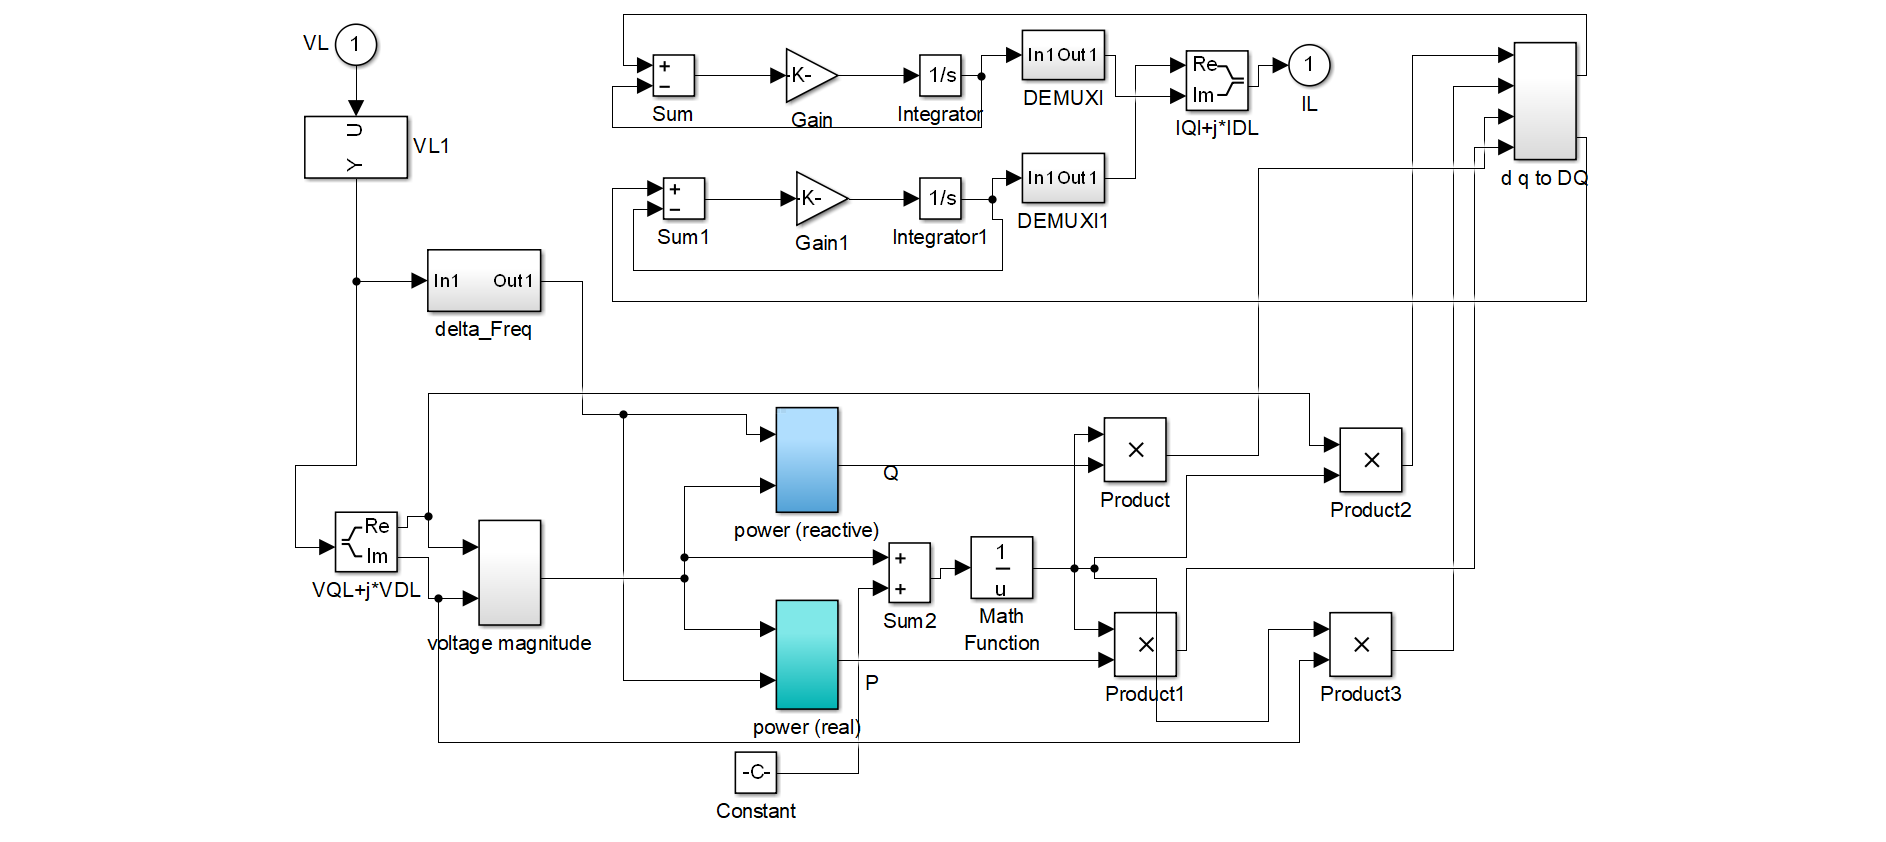
\includegraphics[scale=0.4]{Static Loads}
	\caption{Static Load Model}
	\label{Static Load Model}
	\end{figure}
	
%	% Static Load Sub Models-------------------------------------------------
%	\begin{itemize}
%	\item \textbf{\large Static Load Sub Models}: Static Load Model includes Voltage Magnitude, Real and Reactive Power models to calculate the consumption.
%		\begin{figure}[H]
%		 \centering
%		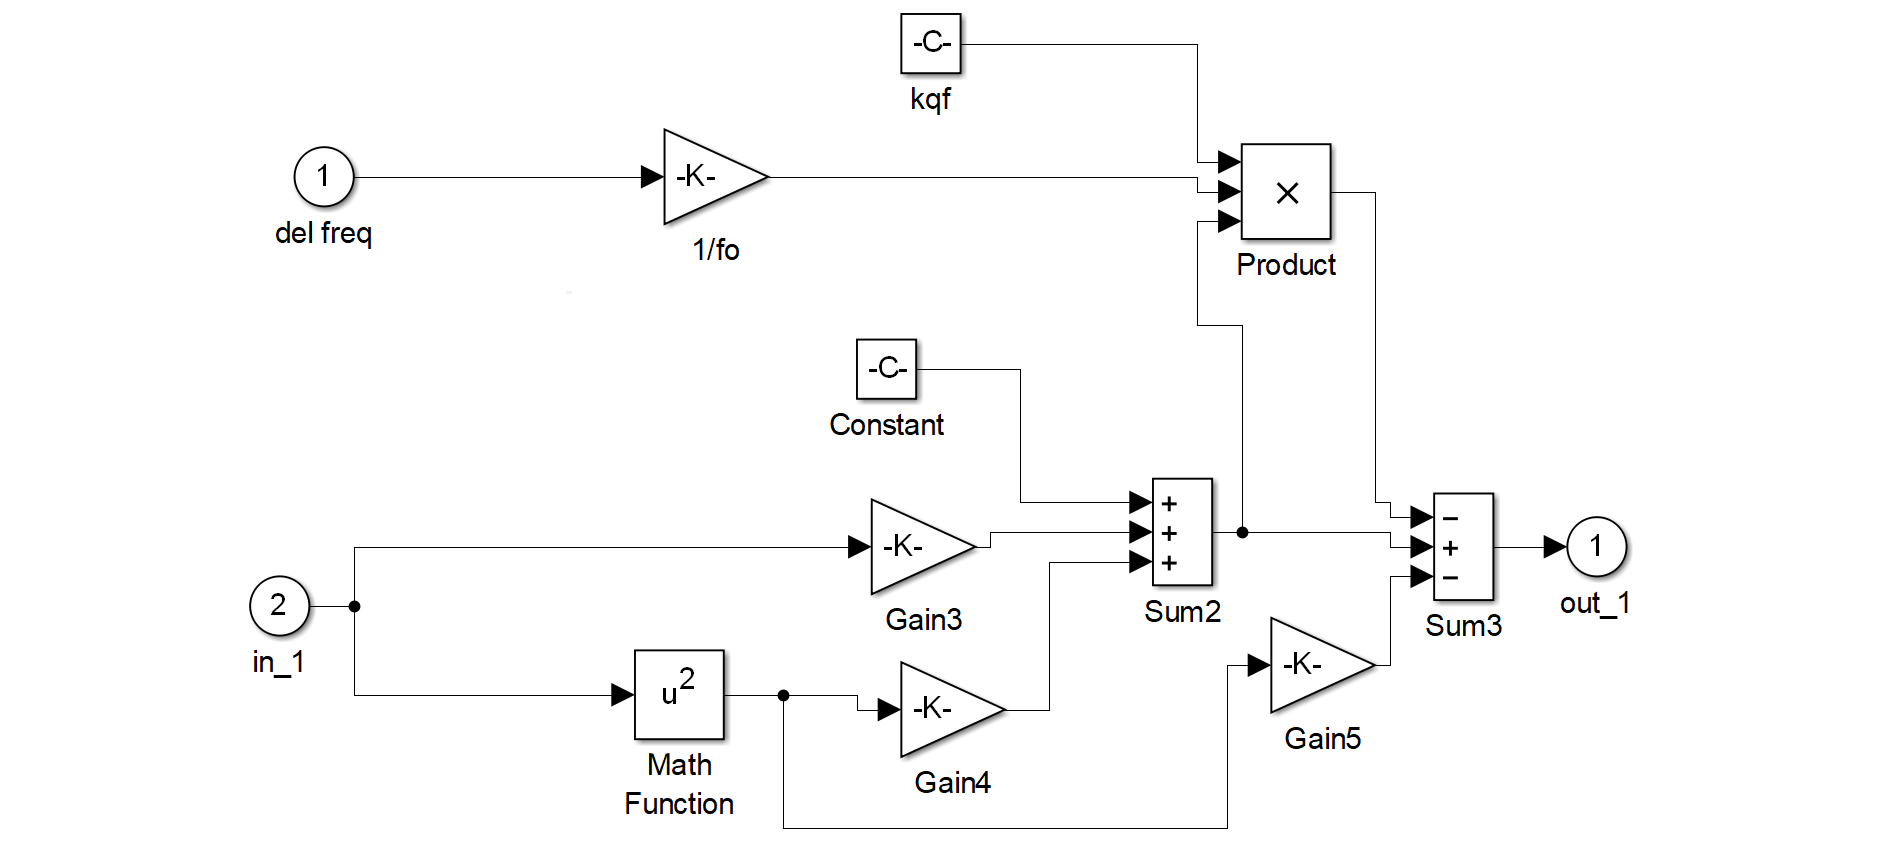
\includegraphics[scale=0.3]{Reactive Power}
%		\caption{Reactive Power Model}
%		\label{Reactive Power}
%		\end{figure}
%		
%		\begin{figure}[H]
%		 \centering
%		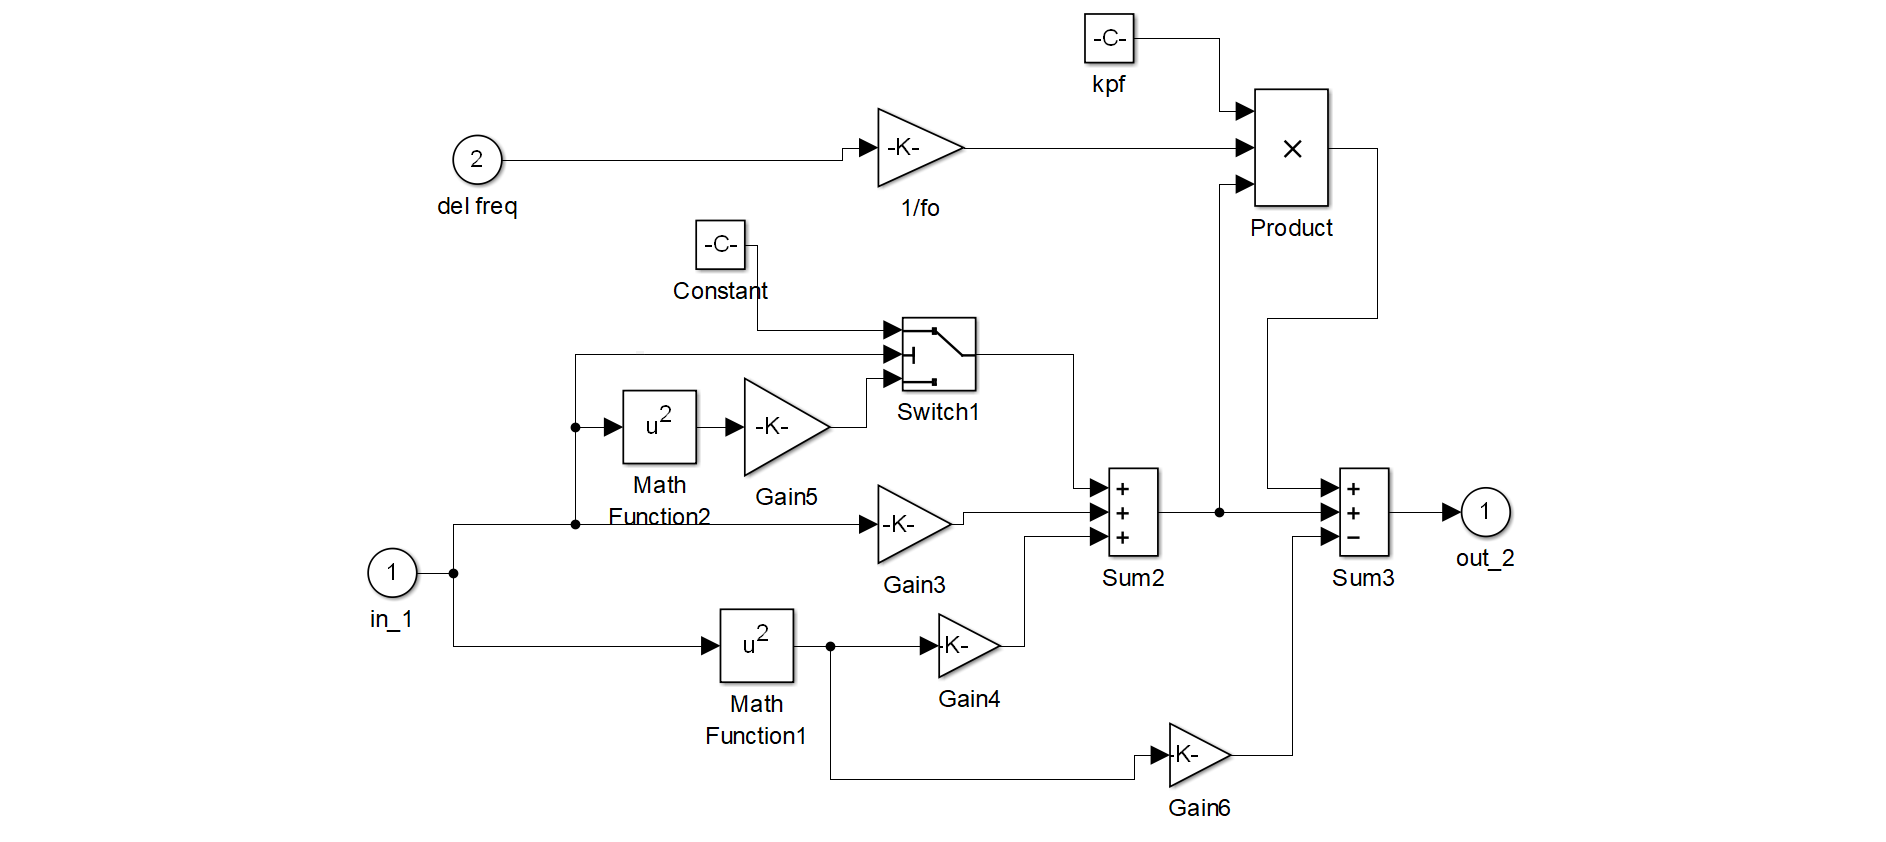
\includegraphics[scale=0.3]{Real Power}
%		\caption{Real Power Model}
%		\label{Real Power}
%		\end{figure}
%		
%		\begin{figure}[H]
%		 \centering
%		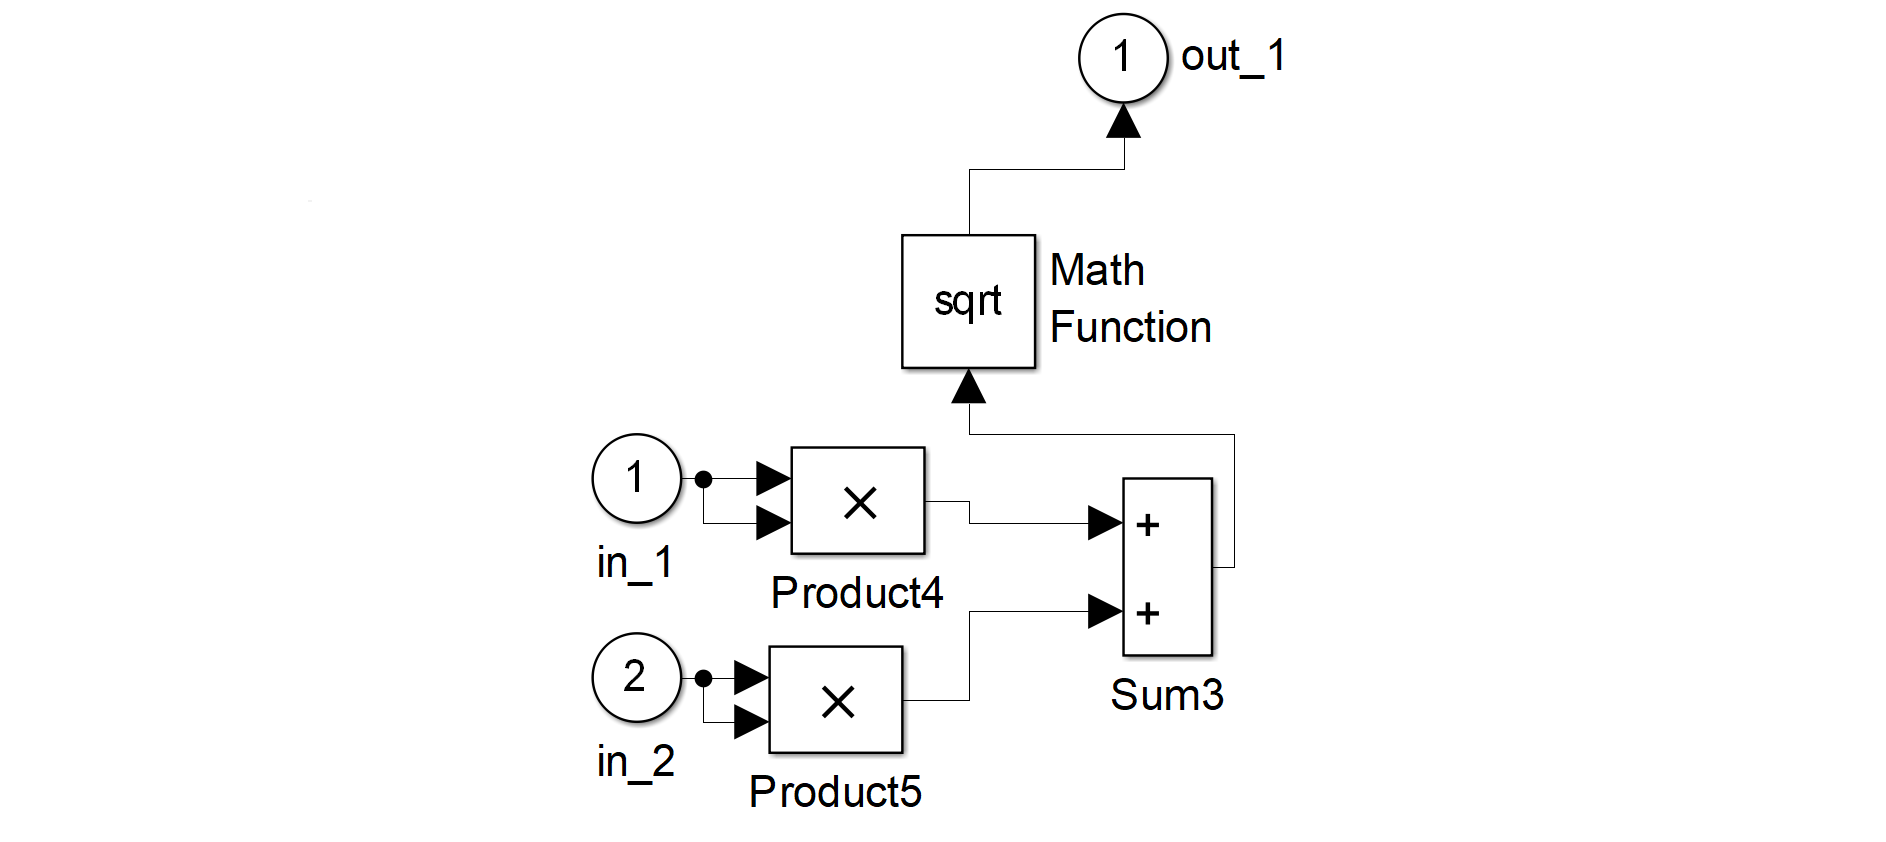
\includegraphics[scale=0.3]{Voltage Magnitude Calculation}
%		\caption{Voltage Magnitude Calculation}
%		\label{Voltage Magnitude Calculation}
%		\end{figure}
%		
%	\end{itemize}	

%% 5. PSS Model===================================================	
\item \textbf{\large Power System Stability Model}: It is created to give feedback to the excitation system according to the deviation of generator from the system parameters. It checks the generator slip and torque and bus voltage and by using four functions (Slip Signal, Power Input, Frequency Input and DelP\_Omega) it gives the feedback voltage.  
	
	\begin{figure}[H]
	 \centering
	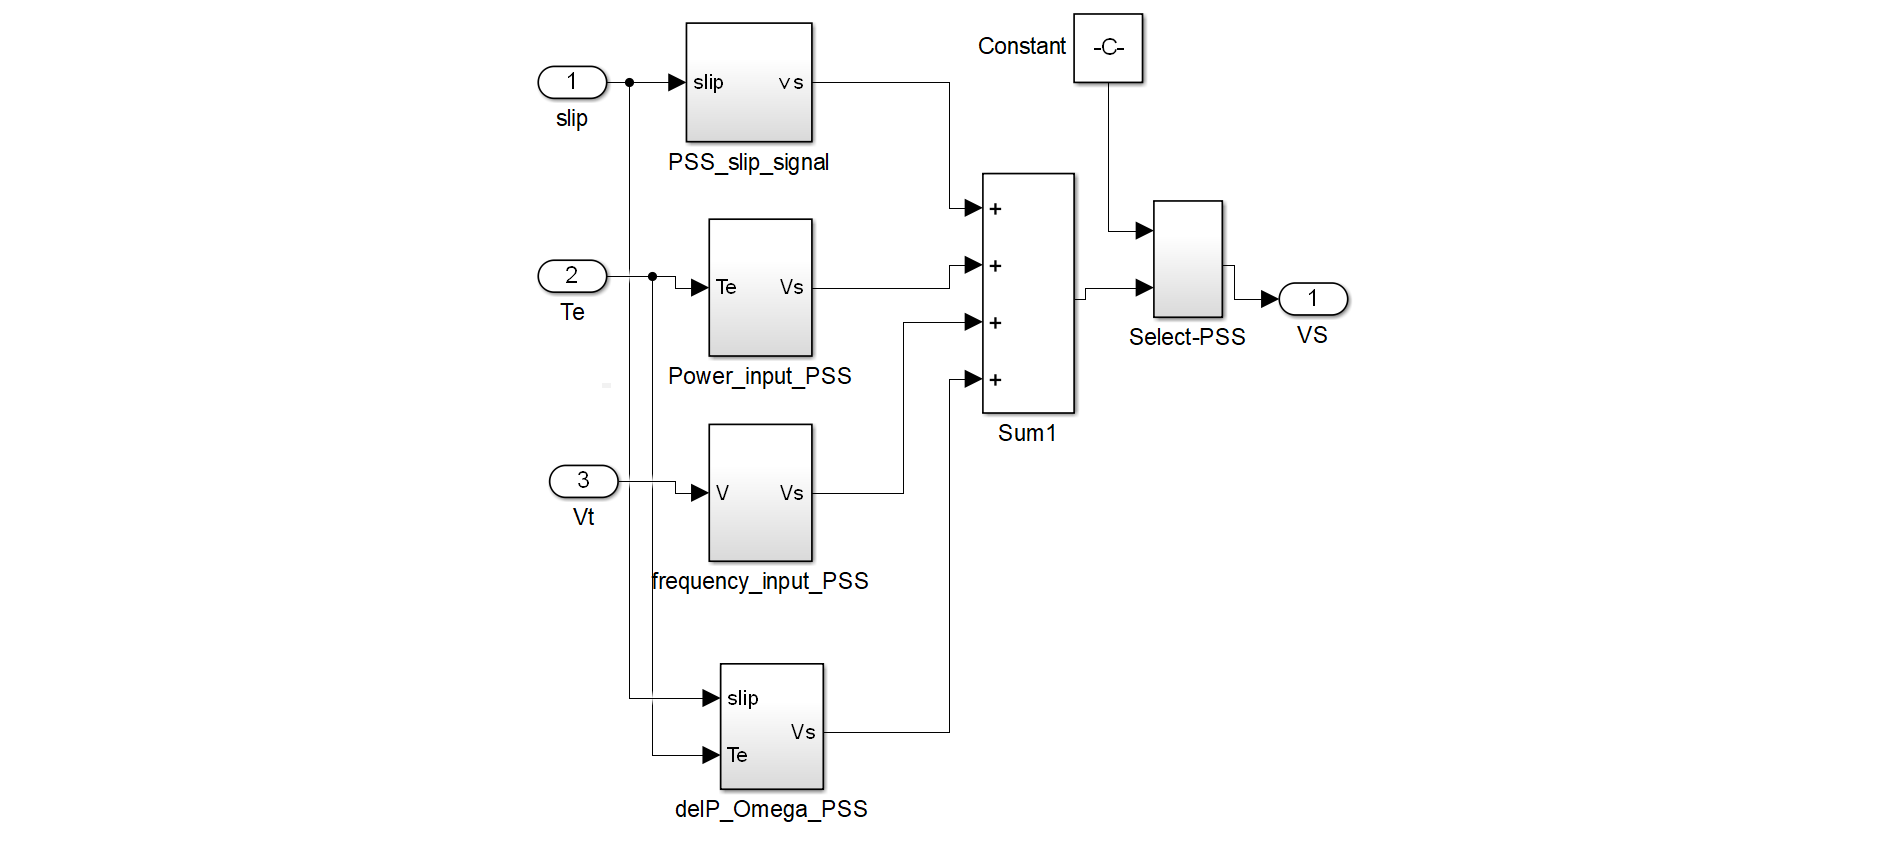
\includegraphics[scale=0.4]{PSS}
	\caption{Power System Stability Model}
	\label{Power System Stability Model}
	\end{figure}
	
%	% PSS Sub Models-------------------------------------------------
%	\begin{itemize}
%	\item \textbf{\large Power System Stability Sub Models}: Static Load Model includes Voltage Magnitude, Real and Reactive Power models to calculate the consumption.
%		\begin{figure}[H]
%		 \centering
%		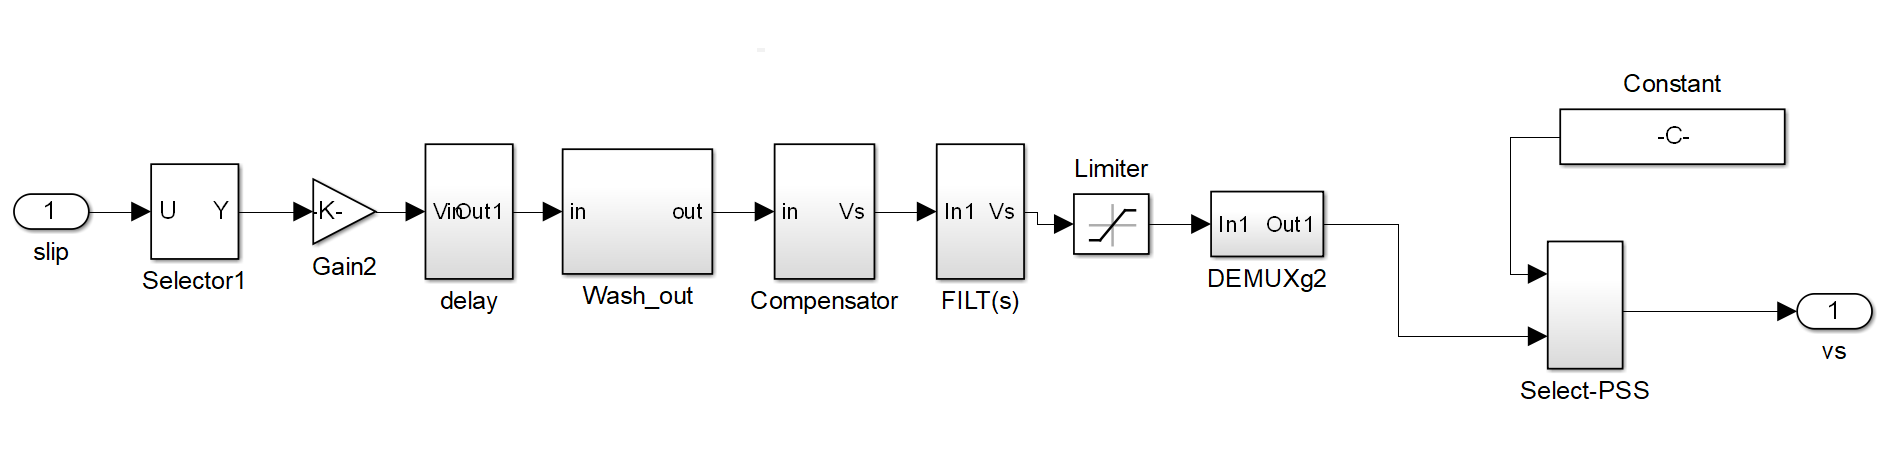
\includegraphics[scale=0.3]{Slip Signal PSS}
%		\caption{Slip Signal PSS}
%		\label{Slip Signal PSS}
%		\end{figure}
%		
%		\begin{figure}[H]
%		 \centering
%		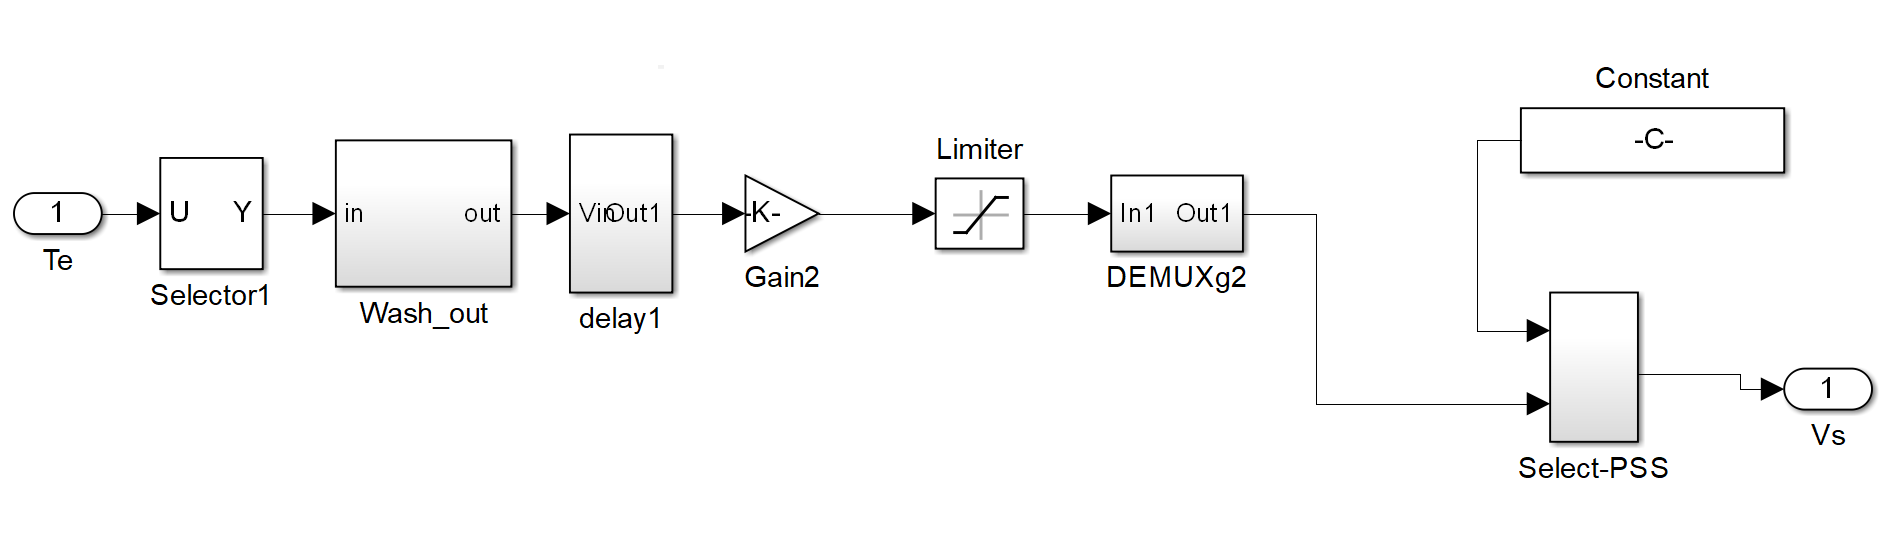
\includegraphics[scale=0.3]{Power Input PSS}
%		\caption{Power Input PSS}
%		\label{Power Input PSS}
%		\end{figure}
%		
%		\begin{figure}[H]
%		 \centering
%		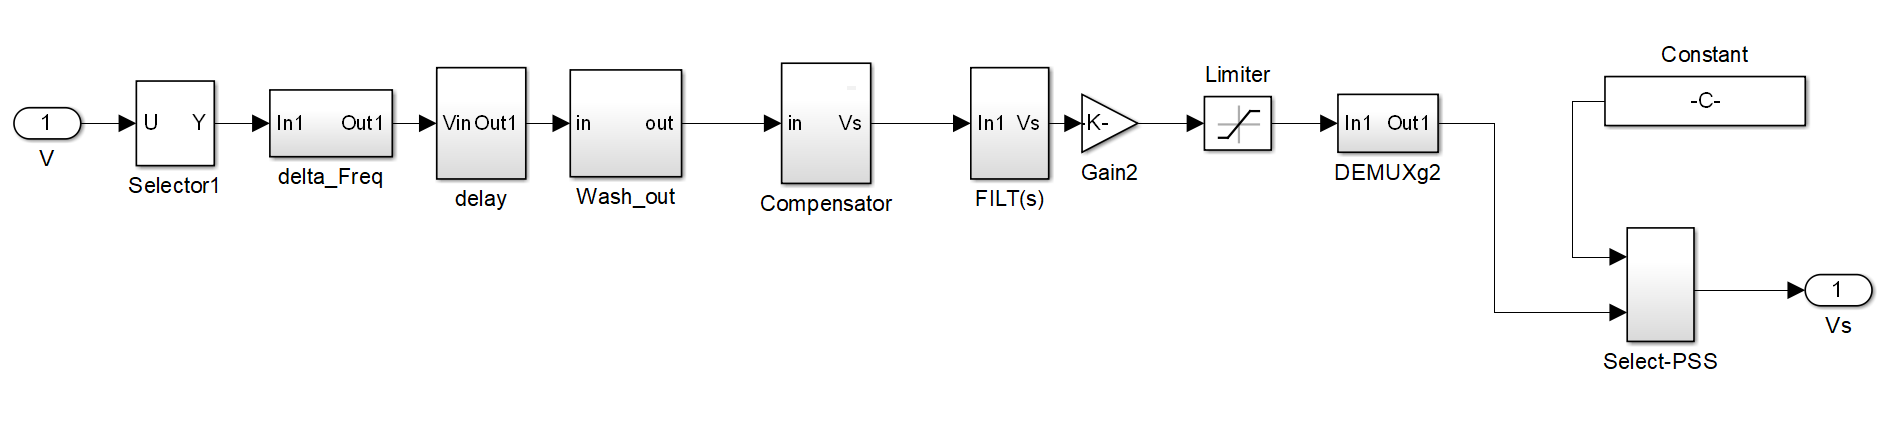
\includegraphics[scale=0.3]{Frequency Input PSS}
%		\caption{Frequency Input PSS}
%		\label{Frequency Input PSS}
%		\end{figure}
%		
%		\begin{figure}[H]
%		 \centering
%		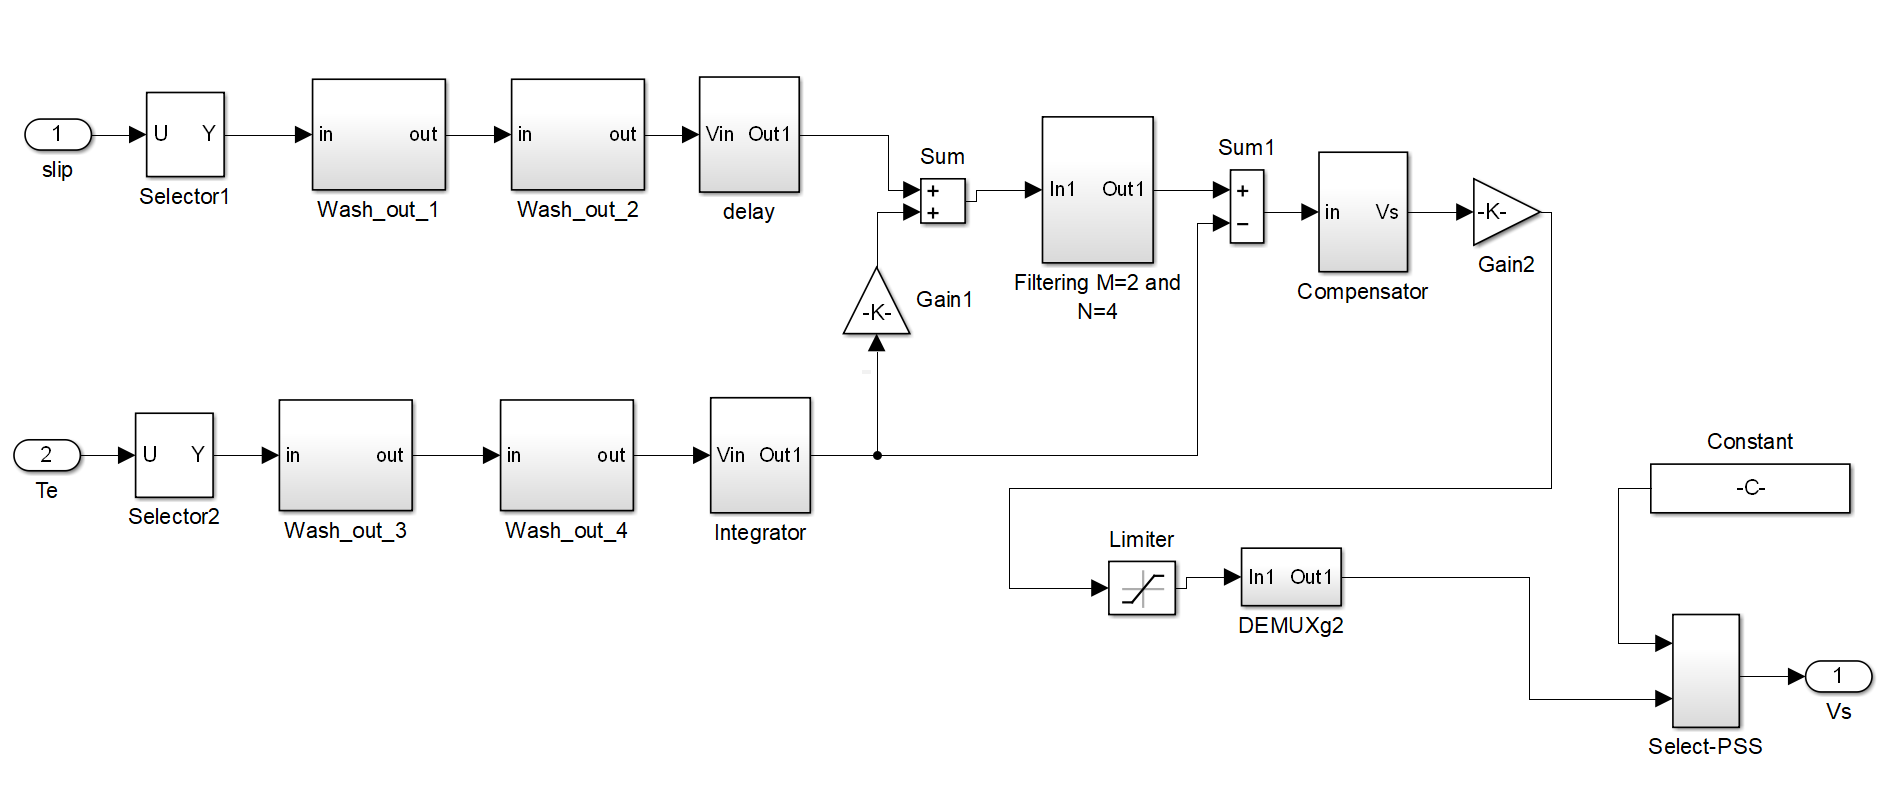
\includegraphics[scale=0.3]{delP Omega PSS}
%		\caption{DelP Omega PSS}
%		\label{delP Omega PSS}
%		\end{figure}
%	\end{itemize}	

%% 6. OUTPUT Model===================================================	
\item \textbf{\large System Parameters Output in Scope}: 8 System parameters (Generator Angle Deviation, Field EMF, Quadrature Axis Parameter, Direct Axis Parameter, Field Current, Mechanical Torque, Electrical Torque and System Voltage) are loaded to observe the result of transient stability of the system in graphical form.
	
	\begin{figure}[H]
	 \centering
	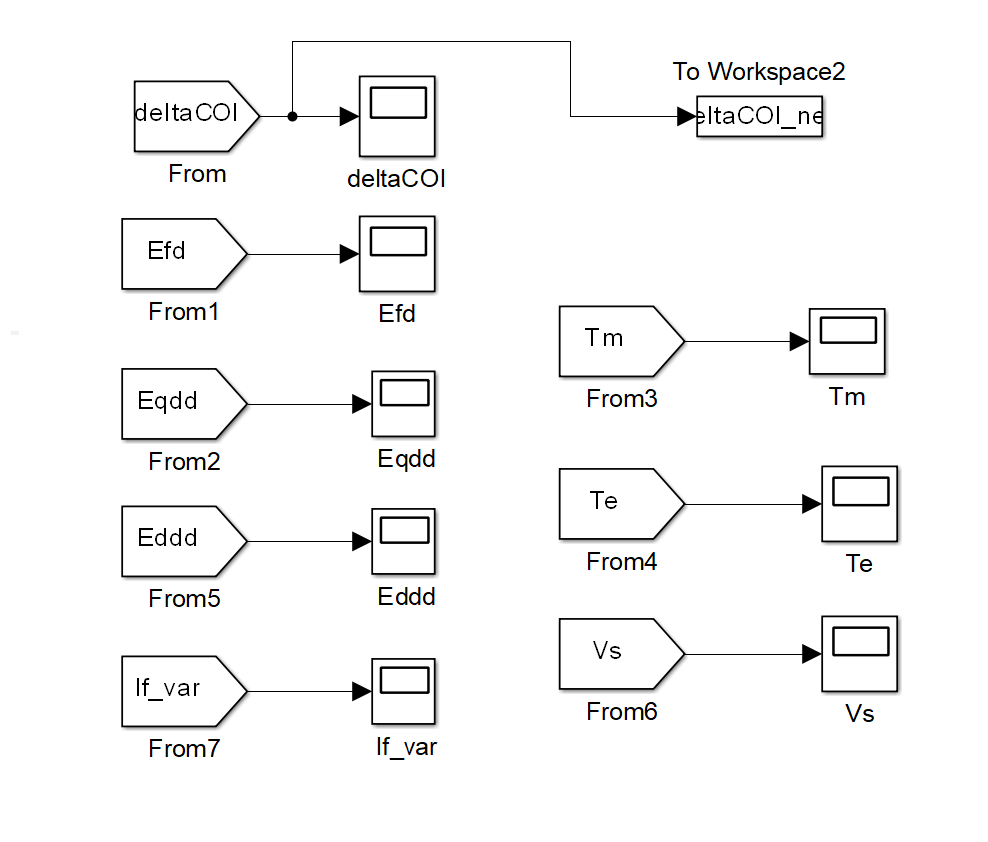
\includegraphics[scale=0.4]{output}
	\caption{System Parameters Output}
	\label{System Parameters Output}
	\end{figure}	
	
	
\end{enumerate}


\section{Computation of Indicators}
As Indicators are described before in section \ref{Catastrophic Indicators} briefly are used for analysing stability of the system after it experiences any type of fault. Generalized formulas of indicators (eqn. \ref{IS} to eqn. \ref{IL}) use system parameters shown in fig. \ref{System Parameters Output} to evaluate itself are used for evaluating the system stability. Analysis of Indicator has a main role of threshold values, which describe the system is stable or not. Selection of threshold vales depend upon the operator looking into the system parameters. Threshold vales are generally obtained from optimization or training Decision Trees. Threshold values are different for different type of contingencies. The proposed Catastrophic Indicators are summarized in Table \ref{Indicators}. These equations are solved and compared with threshold values to decide a system is table or not. The procedure of computation of Indicators is described in Algorithm \ref{Computation of Indicators}.

\begin{table}[!tb]

\renewcommand{\arraystretch}{2}
\caption{Proposed Catastrophic Indicators}
\label{Indicators}
%\begin{center}
\begin{tabular}{|P{0.2\linewidth} | P{0.8\linewidth}|}
\hline
 \textbf{NAME} & \textbf{INDICES}  \\ \hline
 Indicator based on Coherency & $Performance \; Index = max(max(\theta_i(t))-min(\theta_i(t)))$  \\ \hline
 Indicator based on Transient Energy Conversion & $Performance \; Index = max(max(|V_{ke}(t) - V_{pe}(t)|))$ \\  \hline 
 Indicator based on Dot Products (CSA) & $v(t) = \sum_{i=1}^{N_{area}} \omega_i(t)[\delta_i(t) - \delta_i(0^+)]$   \\ \hline
 Wide Area Severity Index (WASI) & $Fast WAST(T) = log(max_{t \; \in \; [0^+,T]}(max_i(PSD(V_i(t)))))$ \\  \hline 
 Inter-area Stability Prediction Index (ISPI) & $SPI = 1-(1-P\Delta V).(1-PV').(1-P\Delta d \delta gc).(1-Pd \delta gc') $ \\ \hline
\end{tabular}
%\end{center}
\end{table}

\begin{algorithm}[H]
\caption{Computation of Indicators}
\label{Computation of Indicators}
\begin{algorithmic}
\While {(a case in possibility dataset isn't handled)}
\begin{itemize}
    \item[--] Get the voltage and phase angle of all buses, as well as areawise and systemwise coherency measures, for the conceivable case.
\end{itemize}
\While {(an indicator isn't handled)}
\begin{itemize}
    \item[--] Figure the indicator values for the 20 ms (50 Hz)
time-stepped information of possibility case
    \item[--] Examine the strength condition in terms of its maximum value and label the instance as stable or unstable.
    \item[--] Update the case with the Indicator name and the condition of its soundness.
\end{itemize}
\EndWhile
\State \textbf{end while}
\EndWhile
\State \textbf{end while}
\end{algorithmic}
\end{algorithm}